\documentclass[UKenglish, thumbmarks]{uiophdthesis}
\usepackage[utf8]{inputenc}
\usepackage[T1]{fontenc}
\usepackage{babel}
\usepackage{amsmath}
\usepackage{amssymb}
\usepackage{array}
\usepackage{graphicx}
\usepackage{textcomp}
\usepackage{url}
\urlstyle{sf}
\usepackage[hidelinks,hypertexnames=false]{hyperref}
\hypersetup{
  pdftitle={Long-Range Dependency Learning in Graph Neural Networks: Benchmarks, Explanations, and Limits},
  pdfauthor={Dongzhuoran Zhou},
  pdfsubject={PhD thesis},
  pdfkeywords={graph neural networks, long-range dependencies, benchmark design, GLoRa}
}
\newcolumntype{L}[1]{>{\raggedright\arraybackslash}p{#1}}

\title{Long-Range Dependency Learning in Graph Neural Networks}
\subtitle{Benchmarks, Explanations, and Limits}
\author{Dongzhuoran Zhou\\ \url{dongzhuz@student.matnat.uio.no}}

\begin{document}

\maketitle[
  dept={Department of Informatics},
  fac={Faculty of Mathematics and Natural Sciences},
  supervisors={Egor V. Kostylev and Evgeny Kharlamov},
  year={2026}
]

\frontmatter

\begin{abstract}
Graph neural networks usually compute node representations by passing messages between neighbouring nodes.
This local mechanism makes learning difficult when the label of a target node depends on information many hops away.

Falling accuracy as dependency length increases does not by itself show which dependency a system learned or why its performance fell.
A benchmark may also permit shortcut functions that fit its examples without using the intended dependency.

GLoRa is a synthetic benchmark generator for inductive binary node classification, parameterised by dependency length.
For any chosen precision and probability, GLoRa provides a corresponding sample-size condition under which, with at least that probability, every function fitting the generated sample relies on the intended path-aware dependency to that precision.
The model family under evaluation can nevertheless express a function that fits the examples.

Many tested systems lose accuracy as the generator's dependency-length parameter increases.
In the setting examined, the reported diagnostics do not support treating over-smoothing, the tested directed-path account of over-squashing, or vanishing weight gradients as complete explanations.

These results provide controlled evidence for one family of long-range dependencies, not a universal account of long-range graph learning.
\end{abstract}

\begin{xabstract}[Sammendrag]
Grafnevrale nettverk beregner vanligvis noderepresentasjoner ved lokal meldingsutveksling mellom nabonoder.
Denne lokale mekanismen skaper en utfordring når etiketten til en målnode avhenger av informasjon mange hopp unna.

Et fall i nøyaktighet når avhengighetslengden øker, viser ikke i seg selv hvilken avhengighet et system har lært eller hvorfor ytelsen faller.
En benchmark kan også åpne for snarveier: funksjoner som gir riktige svar på eksemplene uten å bruke den tilsiktede avhengigheten.

GLoRa er en generator for syntetiske benchmarker innen induktiv binær nodeklassifisering, med avhengighetslengde som parameter.
For ethvert valgt presisjonsnivå og sannsynlighetsnivå gir GLoRa en tilhørende betingelse på utvalgsstørrelsen.
Når betingelsen er oppfylt, gjelder det med minst den valgte sannsynligheten at enhver funksjon som gir riktige svar på det genererte utvalget, er avhengig av den tilsiktede stiavhengigheten med den valgte presisjonen.
Modellfamilien som evalueres, kan likevel representere en slik funksjon.

Mange av de testede systemene får lavere nøyaktighet når generatorens parameter for avhengighetslengde øker.
I det undersøkte eksperimentelle oppsettet gir de rapporterte diagnostiske analysene ikke tilstrekkelig støtte til å anse over-smoothing eller forsvinnende vektgradienter som fullstendige forklaringer.
Det samme gjelder den testede forklaringen på over-squashing, som bygger på rettede stier.

Resultatene gir et kontrollert empirisk grunnlag for å vurdere læring innenfor én familie av langtrekkende avhengigheter.
De gir ikke en universell forklaring på læring av langtrekkende avhengigheter i grafer.
\end{xabstract}

\begin{preface}
This thesis was written at the Department of Informatics, University of Oslo, under the supervision of Egor V. Kostylev and Evgeny Kharlamov.
I am grateful to my supervisors for their guidance, feedback, and support throughout my work on GLoRa and this thesis.
I also thank my collaborators and colleagues for the discussions that helped shape the ideas presented here.

This article-based thesis comprises a kappa followed by one included paper.
\end{preface}

\tableofcontents
\listoffigures
\listoftables

\chapter*{List of Papers}
\addcontentsline{toc}{chapter}{List of Papers}

\begin{description}
\item[Paper I]
Dongzhuoran Zhou, Evgeny Kharlamov, and Egor V. Kostylev.
\emph{GLoRa: A Benchmark to Evaluate the Ability to Learn Long-Range Dependencies in Graphs}.
Published as a conference paper at ICLR 2025.
\end{description}

\chapter*{Author Contribution}
\addcontentsline{toc}{chapter}{Author Contribution}

Dongzhuoran Zhou is the first author of Paper I.
The kappa synthesises the contribution of Paper I within the broader thesis.

\mainmatter

\chapter{Introduction}

\section{Long-Range Graph Learning as an Evaluation Problem}

Consider a target node whose binary label depends on a source node several edges away.
The source feature alone is not sufficient because the label also depends on the intermediate nodes along a source-to-target path.
A positive case contains the required feature pattern along that path, whereas a plausible negative case preserves the distant source and target but breaks the path condition at an intermediate node.
Distinguishing these cases for the intended reason requires a path-aware dependency rather than mere access to a distant node.

\begin{figure}[t]
\centering
\begin{minipage}[t]{0.49\textwidth}
\centering
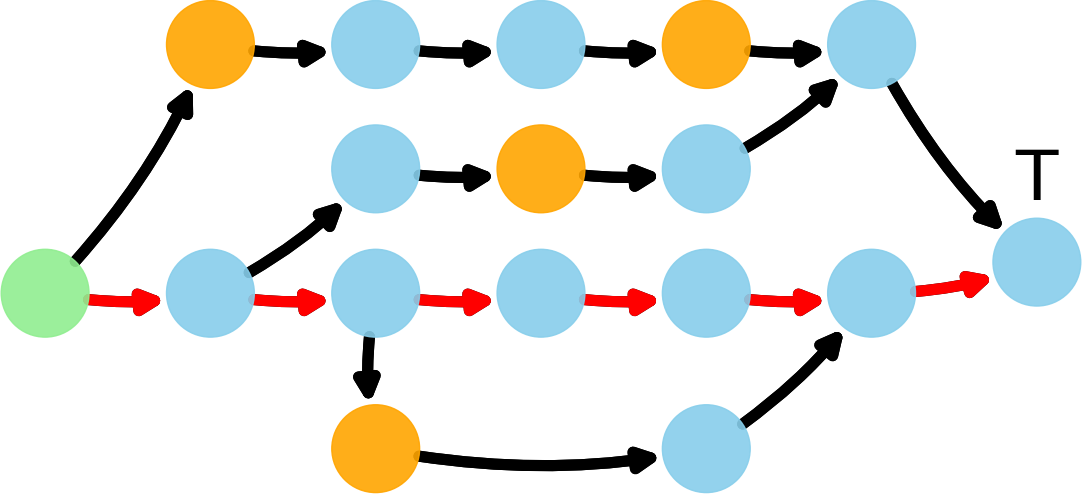
\includegraphics[width=\linewidth]{figures/glora-positive-d6.png}
\textbf{(a)} Positive example
\end{minipage}\hfill
\begin{minipage}[t]{0.49\textwidth}
\centering
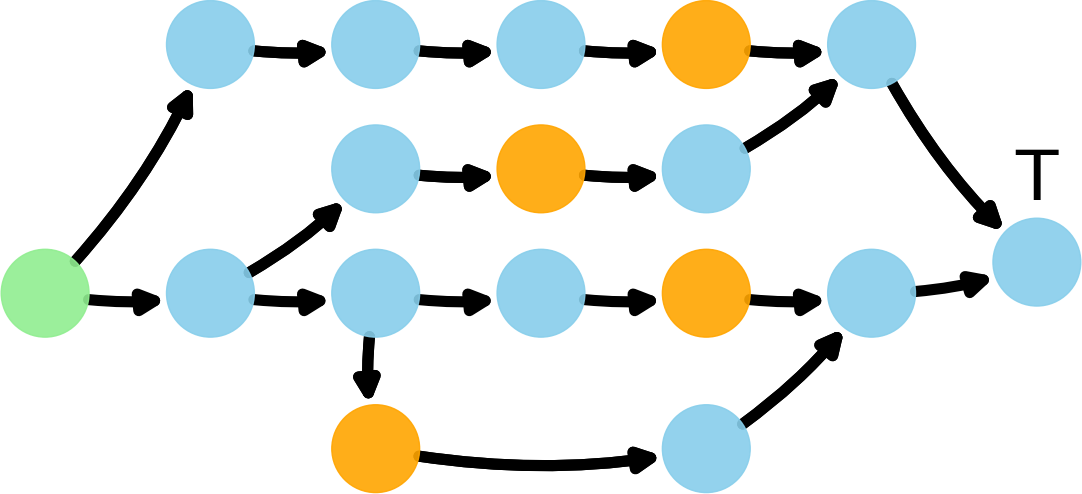
\includegraphics[width=\linewidth]{figures/glora-negative-d6.png}
\textbf{(b)} Negative example
\end{minipage}
\caption{A positive and a negative GLoRa example at generator parameter $d=6$.
Green nodes mark sources, blue nodes are normal nodes, orange nodes are holes, and $T$ marks the target node.
The red arrows identify the intended source-to-target chain; the negative example breaks this chain with a hole.
Adapted from Figure~1 of Paper~I \cite{zhou2025glora}.}
\label{fig:glora-running-example}
\end{figure}

This example also exposes an ambiguity in benchmark evidence.
A graph learning system may predict the labels from the source-to-target relation, or it may use a local marker or global statistic that happens to correlate with the labels.
Both functions can produce high accuracy on a dataset that permits the shortcut.
The score alone therefore does not show which function the system learned.

This distinction matters because graph learning is used when relations between objects carry information that isolated feature vectors omit.
Long-range relations arise in social influence and recommendation \cite{qiu2018deepinf,fan2019graph,liu2022social}, traffic and air-quality prediction \cite{li2021traffic,iskandaryan2023air}, internet safety and finance \cite{han2020fake,weber2018aml}, and biochemical prediction \cite{jha2022protein,bongini2022drugnn}.
These applications do not share one target function or one useful notion of distance.
They do share the need to establish whether a prediction used relevant information beyond the target node's immediate neighbourhood.

Message-passing graph neural networks provide the main technical setting for this problem \cite{scarselli2008graph}.
Their local updates make information from progressively more distant nodes available as layers are added.
Availability does not establish use: a source node may fall inside the receptive field while the learned prediction ignores the source-to-target path.
The modelling problem is to make the relevant information available and learnable, while the evaluation problem is to show that the learned function depends on it.

A benchmark for this purpose must specify the intended dependency and vary its length under controlled conditions.
It must also rule out shortcut functions, keep the target function expressible by the evaluated systems, and compare the two classes fairly.
Without these controls, success may overstate long-range ability and failure may reflect an inexpressible target rather than a learning limitation.

This thesis responds to that evaluation gap through GLoRa, the Graph Long-Range dependency benchmark introduced in the sole included paper \cite{zhou2025glora}.
GLoRa is a synthetic benchmark generator that treats dependency length as a controlled input to inductive binary node classification.
It addresses one family of path-aware dependencies and links a benchmark score to evidence about whether a system learned the specified dependency.
The thesis therefore uses GLoRa as a controlled evaluation method rather than only as a leaderboard.

\section{Scope and Research Questions}

The thesis has a deliberately narrow empirical scope.
It studies inductive binary node classification and one controlled family of path-aware dependencies.
Each example contains a graph, a target node, and a binary label, while the relevant evidence concerns a source-to-target relation of specified length.
The thesis does not claim that this setting represents every node-level, graph-level, or real-world long-range task.

The scope also separates quantities that can otherwise be conflated.
Graph size does not determine dependency length, and access at a large graph distance does not by itself demonstrate the intended dependency.
Later chapters distinguish the exact witness-path length from the implemented GLoRa generator parameter whenever their values differ.
Here, dependency length names the property under evaluation; it does not mean graph size or model depth.

The thesis does not infer a mechanism from an accuracy curve.
An accuracy trend is an observed symptom that requires separate diagnostic evidence before it supports a failure explanation.
Chapter 4 examines over-smoothing, over-squashing, and vanishing gradients as candidate explanations.

Within these boundaries, the thesis addresses three research questions.

\begin{description}
\item[RQ1:]
What evidence is required to conclude that a graph learning system has learned a path-aware dependency of a specified length?

\item[RQ2:]
How can a benchmark isolate a path-aware dependency of a specified length while ruling out shortcut functions, retaining target expressibility, and comparing systems fairly?

\item[RQ3:]
Under controlled evaluation, how does performance change with dependency length, and to what extent do the diagnostics support common failure explanations?
\end{description}

RQ1 defines the evidential claim, and RQ2 asks how an evaluation can support it.
RQ3 then asks what the resulting measurements establish within the tested setting.

\section{Contributions and Paper I}

This is an article-based thesis with one included paper.
Paper I is the thesis's sole empirical contribution and the paper around which the kappa is organised.

\begin{description}
\item[Paper I]
Dongzhuoran Zhou, Evgeny Kharlamov, and Egor V. Kostylev.
\emph{GLoRa: A Benchmark to Evaluate the Ability to Learn Long-Range Dependencies in Graphs}.
Published as a conference paper at ICLR 2025.
\end{description}

Dongzhuoran Zhou is the first author of Paper I.

The thesis makes three contributions through Paper I and the kappa.

\begin{enumerate}
\item \textbf{An evidence standard for path-aware long-range learning (RQ1).}
This contribution states what must be shown before a benchmark result supports a claim about a dependency of specified length.
It draws on GLoRa's path-aware definition and the locality, expressivity, and access-versus-use analysis in Chapters 2 and 3 \cite{zhou2025glora}.

\item \textbf{A controlled benchmark for the stated dependency family (RQ2).}
GLoRa is a generator for evaluating inductive binary node classification across controlled dependency lengths.
Its construction and formal guarantees define the path-aware dependency, rule out shortcut functions under the stated conditions, establish target expressibility, and specify the fairness conditions \cite{barcelo2020logical,zhou2025glora}.

\item \textbf{A controlled comparison and diagnostic assessment across dependency lengths (RQ3).}
This contribution compares graph learning systems under controlled conditions and assesses candidate failure explanations.
It combines experiments indexed by dependency length with separate diagnostics for over-smoothing, over-squashing, and vanishing gradients in Paper I \cite{zhou2025glora}.
\end{enumerate}

These contributions stop at the tested systems, protocol, and path-aware dependency family.
They do not provide a universal account of long-range graph learning or identify a general cause of failure.

\section{Research Questions, Chapters, and Evidence}

Table~\ref{tab:introduction-rq-evidence} maps each research question to the chapters that develop it and to the corresponding form of evidence in GLoRa.

\begin{center}
\centering
\begin{tabular}{L{0.12\textwidth}L{0.40\textwidth}L{0.34\textwidth}}
\hline
\textbf{RQ} & \textbf{Kappa chapters} & \textbf{Evidence from GLoRa} \\
\hline
RQ1 & Chapters 2 and 3 & GLoRa definition \\
RQ2 & Chapters 5 and 6 & Construction, Properties~(P1)--(P3), length control, and protocol controls \\
RQ3 & Chapters 4 and 6 & Length-indexed performance and diagnostics \\
\hline
\end{tabular}
\captionsetup{hypcap=false}
\captionof{table}{Research questions, kappa chapters, and evidence from GLoRa.}
\captionsetup{hypcap=true}
\label{tab:introduction-rq-evidence}
\end{center}

For RQ1, Chapter 2 establishes when local message passing can access distant information, and Chapter 3 states what would demonstrate use of a path-aware dependency.
GLoRa's path-aware definition fixes the dependency to which this evidence standard applies.

For RQ2, Chapter 5 derives the benchmark requirements from threats to interpretation, and Chapter 6 shows how the GLoRa construction addresses those requirements.
The construction and its formal guarantees cover controlled dependency length, the stated shortcut exclusions, target expressibility, and class-distribution fairness; separate evaluation controls provide system-protocol fairness.

For RQ3, Chapter 4 states what evidence candidate explanations require, and Chapter 6 presents the length-indexed experiment and the corresponding diagnostics.
The performance trend is therefore only a symptom; the diagnostic measurements provide the evidence for assessing an explanation.

\section{Thesis Structure}

Chapter 2 establishes the graph-learning foundations needed to interpret a claim about long-range use, including local message passing, receptive fields, and expressivity.
Chapter 3 then distinguishes reachable information from information used by a prediction and develops the path-aware evaluation target and evidence standard for RQ1.

Chapter 4 identifies the diagnostic trace required for each candidate failure explanation.
Chapter 5 reviews whether existing evaluations control shortcut functions, target expressibility, fair comparison, and dependency length.

Chapter 6 presents GLoRa's construction, experiments, and diagnostics for RQ2 and RQ3.
Chapter 7 answers the three research questions, then discusses limitations and future work within the same evidence boundaries.

\chapter{Technical Foundations}

This chapter fixes the graph-learning concepts used to define long-range dependency learning in later chapters.
The progression starts with graph inputs and learning tasks, then moves from local message passing to receptive-field growth.
It next states the symmetry and expressivity constraints on these models.
The final section separates information that an architecture can reach from information that a fitted model has learned to use.

\section{Graphs, Features, and Learning Tasks}

A graph is written as $G=(V,E,\lambda)$.
Here $V$ is a finite set of nodes, $E\subseteq V\times V$ is a set of directed edges, and $\lambda:V\to\mathbb{R}^{n}$ maps each node to an input feature vector.
Nodes are denoted by $u,v,w\in V$.
The feature of node $v$ is $\lambda(v)$, and $n$ is the input feature dimension.

The edge convention fixes the direction of information flow.
An edge $(u,v)\in E$ means that information can be aggregated from $u$ into $v$.
The incoming neighbourhood of $v$ is therefore
\[
N(v)=\{u\in V\mid (u,v)\in E\}.
\]
An undirected edge between $u$ and $v$ is represented by including both $(u,v)$ and $(v,u)$ in $E$.
The same notation therefore covers directed and undirected graphs without changing the aggregation convention.

Graph structure and node features provide different parts of the input.
The edge set determines which nodes are connected and the directions in which information may travel.
The feature map supplies the values attached to those nodes.
A target function may depend on either part or on their relation.

A directed path of length $d$ is a sequence $p=(v_0,\ldots,v_d)$ such that $(v_{i-1},v_i)\in E$ for every $i$ with $1\leq i\leq d$.
When a path carries information relevant to a target prediction, $v_0$ is the source node and $v_d$ is the target node.
The directed graph distance $\operatorname{dist}_G(u,v)$ is the length of a shortest directed path from $u$ to $v$, when such a path exists.
Path length and graph distance are structural properties of $G$.
Dependency length is instead a property of what the target function requires, as Chapter 3 defines in detail.

Graph learning tasks differ by where the prediction is attached.
Node-level tasks predict a value for a target node, edge-level tasks predict a value for a pair of nodes, and graph-level tasks predict one value for the whole graph.
Node classification assigns a discrete label to a target node, whereas node regression assigns a real-valued output.
Binary node classification has two labels, written as True and False in this thesis.

An inductive task requires a learned rule to generalise to graph instances or target nodes not seen during training.
Each inductive node-classification example may be represented by a graph $G$, a target node $v$, and its label.
This setting differs from transductive node classification, where training and test nodes belong to a graph whose structure is already available during training.
GLoRa, the thesis's only included paper, studies inductive binary node classification \cite{zhou2025glora}.
This scope makes the target node representation the main output used in the chapters that follow.

\section{Message-Passing Graph Neural Networks}

Message-passing graph neural networks compute node representations through repeated local updates \cite{scarselli2008graph}.
Each layer aggregates representations from the incoming neighbourhood and combines the result with the node's previous representation.
The same operation is applied at every node, which lets one set of learned parameters operate on graphs with different numbers of nodes.

Let $h_v^{(\ell)}$ denote the representation of node $v$ after message-passing layer $\ell$.
The initial representation is the input feature:
\[
h_v^{(0)}=\lambda(v).
\]
A generic layer first computes the neighbourhood message
\[
m_v^{(\ell)}=\operatorname{Agg}^{(\ell)}\left(\left\{\!\left\{h_u^{(\ell-1)}\mid u\in N(v)\right\}\!\right\}\right),
\]
where $\left\{\!\left\{\cdot\right\}\!\right\}$ denotes a multiset.
It then updates the node representation by
\[
h_v^{(\ell)}=\operatorname{Upd}^{(\ell)}\left(h_v^{(\ell-1)},m_v^{(\ell)}\right).
\]
The aggregation and update functions usually contain learnable parameters.
The layer index indicates that different layers may use different parameters.
Within a layer, the same aggregation and update functions are used at every node in $V$.

The update equation gives the node direct access to its previous representation.
An alternative convention adds self-loops and aggregates over $N(v)\cup\{v\}$.
Both conventions let a node retain or transform its own information while receiving information from its neighbours.
Under the directed-edge convention, each layer follows the available edges into the target node.

Let $L$ be the number of message-passing layers.
For node classification, a final classifier maps the target node representation to a predicted label:
\[
\hat{y}_v=\operatorname{Cls}\left(h_v^{(L)}\right).
\]
For graph-level prediction, an additional readout first forms a graph representation:
\[
h_G=\mathrm{Readout}\left(\left\{\!\left\{h_v^{(L)}\mid v\in V\right\}\!\right\}\right).
\]
The graph predictor then uses $h_G$ rather than one target node representation.
The node classifier and graph readout differ in where they attach the output, but both rely on the same sequence of local node updates.

\section{Locality and Receptive Fields}

Locality follows directly from the message-passing equations.
After one layer, $h_v^{(1)}$ can depend on $\lambda(v)$ and on the initial features of nodes in $N(v)$.
A second layer can also receive information from nodes with edges into those neighbours.
After $\ell$ layers, $h_v^{(\ell)}$ can depend only on nodes that reach $v$ by a directed path of length at most $\ell$.

This set is the receptive field of $v$ at layer $\ell$.
It is defined recursively by
\[
\mathcal{R}_0(v)=\{v\},
\]
and
\[
\mathcal{R}_{\ell}(v)=\mathcal{R}_{\ell-1}(v)\cup\{u\mid (u,w)\in E\ \textrm{for some}\ w\in\mathcal{R}_{\ell-1}(v)\}.
\]
The representation $h_v^{(\ell)}$ is a function only of the graph and features within $\mathcal{R}_{\ell}(v)$ and of the parameters in the first $\ell$ layers.
This claim follows by induction from the aggregation and update equations.

Each local layer expands the receptive field by at most one directed hop.
If $\operatorname{dist}_G(u,v)=d$ and $L<d$, then $u\notin\mathcal{R}_L(v)$.
Changing $\lambda(u)$ while holding the rest of the input fixed cannot then change $h_v^{(L)}$ or $\hat{y}_v$.
This is a structural limitation of the computation graph rather than a property of training.

When $L\geq d$, the source node $u$ lies inside the target node's receptive field.
The architecture then contains a directed computational route by which $\lambda(u)$ may affect $h_v^{(L)}$.
This condition establishes structural reachability only.
It does not establish that the aggregation and update functions preserve the relevant information or that the classifier uses it.

Depth and dependency length therefore play different roles.
Depth $L$ bounds the structural range of a local message-passing computation.
Dependency length states how far the target function requires relevant information to matter.
A model needs enough depth to reach the required information, but sufficient depth alone does not make the fitted prediction depend on that information.

\section{Symmetry and Expressivity}

Graphs have no canonical node order.
Relabelling the nodes changes their representation in memory but not the underlying graph input.
Node-level outputs should follow this relabelling, while a graph-level output should remain unchanged.

Let $\pi$ be a permutation of $V$.
The relabelled graph $G^\pi$ contains an edge $(\pi(u),\pi(v))$ whenever $(u,v)\in E$, and node $\pi(v)$ receives the feature $\lambda(v)$.
A node predictor $F$ is permutation equivariant when
\[
F(G^\pi)_{\pi(v)}=F(G)_v
\]
for every node $v$ and every permutation $\pi$.
Relabelling the input then relabels the node-level output in the same way.

A graph predictor $R$ is permutation invariant when
\[
R(G^\pi)=R(G)
\]
for every permutation $\pi$.
The graph-level output has no node index, so relabelling must leave it unchanged.

Message passing is equivariant when every node uses the same update function and the aggregation function treats its inputs as a multiset.
Changing the order in which neighbours are stored then leaves each aggregated message unchanged.
Applying a permutation-invariant readout to the final multiset of node representations produces an invariant graph representation.
These symmetry properties let the prediction depend on graph structure and features without depending on storage order.

Expressivity describes which input-output functions a model class can represent.
A target function is expressible by a model class if some setting of the model parameters realises that function.
Expressibility is therefore a property of the model class and target function, not of a particular training run.

Locality gives the first expressivity limit.
The target representation $h_v^{(L)}$ can depend only on the graph structure and features inside $\mathcal{R}_L(v)$.
An $L$-layer local message-passing model therefore cannot express a node-classification function whose output at $v$ changes when only information outside this receptive field changes.
No parameter setting can create a computational route from that information to $h_v^{(L)}$.

Even within the receptive field, a particular architecture may map inputs that the target function must distinguish to the same representation.
An aggregation function can map distinct neighbourhood multisets to the same message.
Once two inputs have produced the same intermediate representation, later layers cannot recover the distinction from that representation alone.
Permutation symmetry also prevents a model from using an arbitrary storage position as a node identifier unless that identifier is supplied as a feature.
Logical and combinatorial analyses formalise related limits on which rooted nodes and graphs message-passing architectures can distinguish \cite{barcelo2020logical}.

Learnability is a separate question.
It asks whether a training procedure can use the available data and finite resources to find parameters that realise or approximate an expressible target function.
If the target function is not expressible, no training procedure can realise it exactly.
Failure to realise it exactly therefore does not test learnability.
If the target function is expressible, successful training is still not guaranteed.
An evaluation intended to isolate learnability must therefore establish expressibility before it interprets training success or failure.

\section{From Reachability to Use}

The preceding definitions separate three claims about a target-node prediction.
Structural reachability asks whether the relevant input lies inside the target node's receptive field.
Expressibility asks whether some parameter setting in the model class can compute the required target function.
Demonstrated use is distinct from learnability: it asks whether the fitted predictor actually depends on the relevant input.

These claims are not equivalent: reachability does not establish expressibility, and expressibility does not establish demonstrated use.
A source node outside $\mathcal{R}_L(v)$ is unreachable by an $L$-layer local model.
A source node inside $\mathcal{R}_L(v)$ is reachable, but the model class may still merge inputs that the target function must distinguish.
Even when the target function is expressible, the training procedure may return parameters whose prediction ignores the source information.

Dependence concerns the behaviour of the fitted function under relevant input changes.
To test this dependence, change the relevant source or path information while holding the rest of the input fixed.
The fitted prediction should change in the way required by the target function.
Architectural depth cannot supply this evidence because depth describes possible information flow rather than the function selected by training.

An accuracy trend as graph distance or dependency length increases is likewise a behavioural symptom.
It may show where a fitted system succeeds or fails under an evaluation protocol, but it does not identify the mechanism responsible for that behaviour.
A mechanism claim requires separate evidence that the model exhibits the internal trace predicted by that mechanism.

Chapter 3 builds on this distinction by defining the path-aware dependency that an evaluation must demonstrate.
It separates graph distance and path length from the dependency length required by the target function.
The premise for that definition is the limit established here: being inside a receptive field does not demonstrate dependence.

\chapter{Long-Range Dependency as an Evaluation Target}

\section{From Distant Information to Demonstrated Dependence}

Some graph predictions require information that is not local to the prediction target.
Graph distance identifies where information lies, but it does not establish whether that information determines the correct output.
A long-range dependency is therefore a property of a label function rather than a property of graph size or distance alone.
The correct output must depend on relevant distant information and, in the path-aware setting studied here, on how that information is connected to the target.

Figure~\ref{fig:glora-running-example} provides a paired example that separates reachability, correlation, and dependence.
Suppose a source node \(v_0\) carries a designated feature and a target node \(v_d\) has label True only when every internal node on a source-to-target path carries a required continuation feature.
Compare this graph with an otherwise identical graph in which the feature of one internal node is changed and the target label is False.
The target remains reachable from the source through the same edges in both graphs, so reachability does not explain the label difference.
The source feature is also present in both graphs, so its presence does not distinguish the labels in this pair.
The change in the correct label is instead tied to the changed path information, which demonstrates dependence under the stated label function.
By contrast, frequent co-occurrence of the source feature and the True label in unpaired data would establish correlation only.

This distinction matters across graph domains in which distant evidence can become relevant through relations.
Examples include social influence, upstream traffic conditions, non-local biochemical interactions, web relations, and transaction chains in anti-money-laundering analysis \cite{zhou2025glora}.
The entities and edges differ across these domains, but the evaluation question is the same: whether the correct output requires information connected across several hops.

\section{Path-Aware Dependencies}

GLoRa gives one formalisation of this requirement through a path-aware dependency \cite{zhou2025glora}.
Let \(f\) be a node-classification function that takes a graph and a target node as input, and let \(G=(V,E,\lambda)\).
Let
\[
p=(v_0,\ldots,v_d)
\]
be a simple directed path of length \(d\).
The nodes on the path are distinct, and \((v_{i-1},v_i)\in E\) for every \(i\) with \(1\leq i\leq d\).
The node \(v_0\) is the source node, \(v_d\) is the target node, and each \(v_i\) with \(0<i<d\) is an internal node.

For every internal node \(v_i\), choose an alternative feature vector \(a_i\neq\lambda(v_i)\).
Let \(G_i\) be the graph obtained by replacing only \(\lambda(v_i)\) with \(a_i\).
For indices \(0<k\leq m<d\), let \(G_{p[k,m]}\) retain \(G\) and add a duplicate of each node from \(v_k\) to \(v_m\).
Each duplicate has the same feature as its original node.
For every edge incident to a node in the segment, \(G_{p[k,m]}\) also adds the corresponding edge with each endpoint in the segment replaced by its duplicate.
Write \(v'_j\) for the duplicate of \(v_j\).
Let \(G_{p[k,m],j}\) replace the feature of \(v'_j\) with \(a_j\), and let \(G_{p[k,m],i,j}\) additionally replace the feature of the original node \(v_i\) with \(a_i\).

The function \(f\) relies on a path-aware dependency of length \(d\) if there exist a graph, path, and alternative vectors as defined above for which the following three conditions hold.
\begin{enumerate}
\item \(f(G,v_d)\neq f(G_i,v_d)\) for every \(i\) with \(0<i<d\).
\item \(f(G,v_d)=f(G_{p[k,m],j},v_d)\) for every \(k,j,m\) with \(0<k\leq j\leq m<d\).
\item \(f(G,v_d)\neq f(G_{p[k,m],i,j},v_d)\) for every \(i,k,j,m\) with \(0<i<d\) and \(0<k\leq j\leq m<d\).
\end{enumerate}

The first condition makes the classification sensitive to the designated perturbation at every internal node on the witness path.
This sensitivity alone does not show that the function uses those nodes as a path because an internal feature could matter for an unrelated reason.
The second condition requires the classification to remain unchanged when the feature of any duplicated node \(v'_j\) in any allowed segment \(p[k,m]\) is replaced by \(a_j\), while the original path remains intact.
The third condition requires the classification to change when the features of any original internal node \(v_i\) and any duplicated node \(v'_j\) in any allowed segment are replaced by \(a_i\) and \(a_j\), respectively; \(i\) and \(j\) need not be equal.
Together, the duplicate-only and joint perturbations tie the classification to an intact source-to-target path rather than to a detached feature test.

This path-aware definition is one formalisation of a long-range dependency rather than a claim that every long-range graph relation has this form.
Other definitions could describe distant-node interactions without a single target node or without making one path the witness.
The path-aware choice is appropriate here because it gives a precise task-level counterpart to the local message-passing computation introduced in Chapter~2.

\section{Distance and Dependency Length}

Graph distance, path length, dependency length, and path-aware dependency name different objects.
For nodes \(u\) and \(v\), the graph distance \(\operatorname{dist}_G(u,v)\) is the length of a shortest directed path from \(u\) to \(v\), when such a path exists.
Graph distance is a structural property of \(G\) and does not involve a label function.

Path length belongs to one particular path.
The path \(p=(v_0,\ldots,v_d)\) has length \(d\) because it contains exactly \(d\) edges, whether or not it is a shortest path between its endpoints.
Consequently, \(\operatorname{dist}_G(v_0,v_d)\) can be smaller than the length of \(p\).

Dependency length belongs to the task.
In the formalisation above, \(d\) is the exact length of a path that witnesses the required dependence of the label function.
Path-aware dependency names this dependence relation, whereas dependency length names the number of edges on its witness path.
Distance alone is not a dependency because it says nothing about whether changing distant information can change the output.

Graph distance, path length, and dependency length can coincide numerically, but any equality between them must be established.
A graph can contain a long path while its labels depend only on local information.
A graph can also have a large diameter without any label depending on a pair of distant nodes.
A chosen witness path can also be longer than the shortest route between its endpoints.
An intended rule that refers to a path of length \(d\) is therefore insufficient if the observed labels can be fitted without using that path.

The exact witness-path length used in this definition must also remain distinct from the length parameter supplied to the GLoRa generator in Chapter~6.
A generator parameter controls a construction, so its relation to the exact length of a witness path in a generated graph must be stated separately rather than assumed.
Within this chapter, \(d\) denotes the exact length of the witness path unless a different role is stated explicitly.

Once dependency length has been defined as a task requirement, an evaluation can vary it under controlled conditions.
This replaces a single score with a performance profile over specified witness-path lengths.
Such a profile describes how far demonstrated use extends under the evaluation conditions without treating distance alone as dependence.

\section{Scope of the Definition}

The three-condition definition is node-level.
Paper I applies the definition to GLoRa's inductive binary node-classification setting, and the paper's formal benchmark guarantee is limited to that setting \cite{zhou2025glora}.
The function \(f(G,v_d)\) assigns the target node one of the labels True and False.
The inductive setting requires the learned rule to apply to new graph instances rather than to memorised node identities in one fixed graph.
Within this thesis, formal claims based on the definition are limited to this setting unless an extension is stated explicitly.

The explicit target node makes the intervention direct.
Changing an internal node tests whether the output at \(v_d\) changes, while the duplicate-segment conditions test whether the output depends on an intact path to that target.
The source, internal nodes, and target therefore have fixed roles in the witness.

Graph-level tasks have no distinguished target node in their output format, but their labels can still depend on path information.
One extension treats the place where path information is assembled before graph readout as a conceptual target.
Another treats the path itself as the witness and asks whether perturbing its internal nodes changes the graph label.
Both extensions preserve the distinction between distant information being present and the output depending on its relation across the graph.

These graph-level extensions are conceptual and are not covered by Paper I's formal node-classification result.
A graph-level label may depend on several source nodes, several readout locations, or redundant witness paths.
The difficulty of learning such a label can therefore depend on the amount and arrangement of relevant information as well as on dependency length.

\section{Access Is Not Demonstrated Use}

Access is an architectural property relative to an input graph.
For a standard message-passing graph neural network, each layer expands the target node's receptive field by one directed hop \cite{scarselli2008graph,kipf2017semi}.
If a model has fewer than \(\operatorname{dist}_G(v_0,v_d)\) layers, the feature of \(v_0\) cannot affect the target representation through ordinary one-hop message passing.
Enough layers remove this structural barrier, but they establish only that the information can reach the target representation.

Demonstrated use is a claim about the learned function.
The learned prediction must respond to the relevant path interventions rather than merely receive the source feature inside its receptive field.
In the paired example above, a system that gives the same prediction after the internal feature changes has access to the source but does not exhibit the required dependence.
The duplicate-only and joint perturbations make this test stronger by checking that the response follows the intact path.

Correlation is weaker than both task dependence and demonstrated use.
A feature can predict the label because it co-varies with the label across the sampled examples, even when changing the relevant path information would leave the learned prediction unchanged.
High accuracy on such examples establishes predictive performance, but it does not by itself identify which information the learned function used.
Paired or intervention-based evidence is needed to separate the intended dependence from label-correlated alternatives.

The same boundary applies to failure.
A decline in accuracy as dependency length increases is a behavioural symptom, not a diagnosis of the mechanism that caused the decline.
The mechanism requires separate internal evidence with a prediction that distinguishes it from other explanations.
Chapter~4 develops that diagnostic standard after the learning target has been fixed.

\section{Evaluation Contract}

An evaluation supports a claim about learning a path-aware dependency of a specified length only when four requirements hold.
First, it must state the target output, the path-aware dependency to be learned, and the exact witness-path length.
Second, the evaluated system must have architectural access to the relevant information, and the target function must be expressible by the evaluated model family \cite{barcelo2020logical,zhou2025glora}.
Third, the evidence must make successful prediction depend on the relevant path changes while holding reachability and label-correlated alternatives fixed.
Fourth, comparisons across dependency lengths and systems must use controlled conditions and must report any distinction between an exact witness-path length and a generator parameter.

Under this contract, successful prediction supports a bounded claim that the learned function uses the specified path-aware dependency in the evaluated setting.
Failure supports only the conclusion that, under those conditions, the evaluation did not show that the system had learned a function with the specified path-aware dependency.
Neither result identifies a failure mechanism from accuracy alone, and neither establishes capability for every form of long-range graph relation.

These four requirements provide the basis for RQ~1.
With the learning target and required evidence fixed, Chapter~4 develops mechanism-specific predicted traces for distinguishing explanations of failure.
Chapter~5 then turns this contract into benchmark criteria, including the control of alternative fitting functions and fair comparison between graph learning systems.

\chapter{Why Long-Range Learning Fails and How Models Address It}

Message passing gives source information a route to a target node, but reachability alone does not make that information useful.
A model must preserve task-relevant distinctions during forward propagation, carry enough relevant information through its communication channels, and learn suitable transformations through optimisation.
These requirements motivate three common explanations of long-range failure: over-smoothing, over-squashing, and vanishing gradients \cite{li2018deeper,alon2021bottleneck,glorot2010difficulty}.

The three explanations concern different internal traces.
Over-smoothing concerns contraction of node representations that removes task-relevant distinctions.
Over-squashing concerns inadequate usable influence from relevant source information even though that information is structurally reachable.
Vanishing gradients concern weak backward signals in the parameters that must learn the required computation.
An accuracy decline as dependency length $d$ grows is compatible with all three mechanisms, but it identifies none of them.

Standard message-passing architectures provide useful comparisons because they vary the local operation while retaining one-hop propagation.
GCN uses normalised neighbourhood averaging, whereas GraphSAGE learns inductive neighbourhood aggregation \cite{kipf2017semi,hamilton2017graphsage}.
GAT learns local attention weights, and GIN uses expressive sum aggregation \cite{velickovic2018gat,xu2019gin}.
SGC instead separates repeated propagation from intermediate non-linear transformations \cite{wu2019sgc}.
These differences can change how information survives each hop, but a local architecture still needs sufficient depth for a source node at graph distance $d$ to affect the target node.
Architectures and interventions appear below only when their design addresses a predicted trace or a separate limitation such as strict under-reaching.

This chapter separates mechanisms from symptoms, diagnostics, and interventions.
Sections 2--4 define each mechanism, state its predicted internal trace, group the methods that target it, and delimit what a successful intervention would establish.
Section 5 explains how the mechanisms interact.
Section 6 turns the resulting distinctions into a bounded diagnostic taxonomy for Chapter 6.

\section{Evidence for a Failure Explanation}

A failure explanation must connect an observed performance symptom to a mechanism inside the learned system.
For a dependency of length $d$, the source information must first lie inside the target node's receptive field.
If the model has too few local message-passing layers, the source has exactly zero influence on the target representation.
This case is strict under-reaching, not over-smoothing, over-squashing, or an optimisation failure.

Once the source is reachable, a diagnosis requires a mechanism-specific trace.
Over-smoothing predicts contraction among representations that must remain distinguishable for the task.
Over-squashing predicts inadequate source-to-target influence because topology, dynamics, finite width, or task-relative mixing limits the available communication.
Vanishing gradients predict that the backward signal becomes too small in the layers or parameters that must learn the dependency.
The trace must be measured in the same regime in which the performance symptom appears.

This evidence standard separates four levels of analysis.
An accuracy curve over $d$ is a performance symptom.
A proposed account such as representation contraction is a candidate mechanism.
A measurement such as projection distance, source-to-target sensitivity, or an early-layer gradient norm is a diagnostic.
A residual connection, rewiring rule, or global-attention layer is an intervention.
Conflating these levels turns a method's motivation into a causal conclusion that the experiment has not established.

An intervention can provide stronger evidence when it targets a predicted trace.
The comparison should hold the task, data, effective dependency, model capacity, and training protocol as constant as possible.
The intervention should change the trace in the predicted direction and improve the task outcome in the same runs.
Even this joint result supports a causal account only under the assumptions of the comparison because most interventions change more than one property of the system.

The diagnostic must also be task-aligned.
A graph-level structural proxy may identify a narrow cut without showing that task-relevant information crosses it.
A representation statistic may show contraction without showing that the contracted direction carries the label.
A parameter-gradient norm may be nonzero even when the update direction does not help learn the intended dependency.
The useful question is therefore not whether a familiar pathology can occur, but whether its predicted trace appears in the failing computation and concerns information needed by the target function.

\section{Over-Smoothing}

\subsection{Definition}

Graph propagation often contracts node-varying components of a representation towards an operator-dependent invariant or low-dimensional subspace.
The graph-smoothing interpretation of GCN makes this effect explicit, while later analyses give sufficient spectral and weight-norm conditions for exponential convergence towards an invariant subspace \cite{li2018deeper,oono2020exponentially}.
Over-smoothing occurs when this contraction removes task-relevant distinctions before the model completes the required computation.
The limiting representation need not be a single constant vector, so over-smoothing is broader than literal equality among all node representations.

The mechanism is task-sensitive.
Finite propagation can denoise features or improve a prediction before further smoothing becomes harmful, as shown in model-specific regression and classification analyses \cite{keriven2022not}.
The same amount of contraction can be harmless for a target that depends on a low-frequency graph signal and destructive for a target that requires a distinction between particular nodes.
Depth is therefore not itself evidence of over-smoothing, and an accuracy decrease with depth is only a symptom.

The mechanism is also measurement-sensitive.
Pairwise Euclidean distances depend on representation scale, while cosine similarity ignores changes in norm.
Distance to a theoretically predicted invariant subspace tests a more specific account than a generic variance statistic.
A task-conditioned probe asks whether the remaining representation still contains the distinction required for prediction.
Each diagnostic supports a different statement about contraction.

\subsection{Predicted Internal Trace}

Over-smoothing predicts progressive convergence in the representations of nodes or examples that the target function requires the model to distinguish.
The trace should strengthen with propagation depth or dependency length under otherwise comparable conditions.
It should appear before the task readout, because the proposed mechanism concerns information lost during message passing rather than only a poorly fitted decision boundary.

Complete collapse and label mixing are not the same trace.
Complete collapse maps the measured representations to one value or to the invariant subspace predicted by the propagation analysis.
Label mixing means that representations from examples with different labels overlap under a chosen projection or summary.
Such overlap can follow from poor feature learning, an unsuitable projection, or a task readout that does not use the available information.
It does not by itself show that repeated graph propagation made node representations converge.

A useful diagnostic panel can combine within-graph pairwise distances, cosine similarities, projection distance to a predicted invariant subspace, and task-conditioned probes.
Layerwise measurements show whether contraction develops before the task fails.
Comparisons across node roles distinguish general graph-wide contraction from loss of a particular source-to-target distinction.
The diagnostic should report the graph operator, normalisation, layer, node set, and scale convention because these choices change the trace being measured.

Attention does not remove the need for this test.
Attention-based graph systems can also contract under explicit assumptions, even though their aggregation weights are learned rather than fixed \cite{wu2023demystifying}.
The relevant question remains whether the learned propagation erases a task-relevant distinction.

\subsection{Model and Intervention Families}

The first response is to make the required depth usable without allowing repeated propagation to dominate the representation.
PairNorm maintains the spread of node representations and directly targets a geometric collapse statistic \cite{zhao2020pairnorm}.
Batch normalisation changes representation geometry and scale, while analyses of linearised GNNs show that normalisation can alter the limiting subspace rather than merely delaying convergence \cite{ioffe2015batch,scholkemper2025residual}.
These methods preserve variation in a general sense, but they do not select the source information that the target function requires.

Stochastic regularisation changes how often the same graph mixing is applied during training.
DropEdge randomly removes edges and can slow repeated smoothing while regularising a deep GNN \cite{rong2020dropedge}.
On a path-dependent task, the same removal can also delete an edge that carries useful information.
Its role must therefore be evaluated against both representation contraction and preservation of the required path.

Residual and dense connections give deep layers access to earlier representations.
DeepGCN-style residual and dense architectures preserve shallow features and provide shorter routes through the computation \cite{li2019deepgcns,he2015resnet}.
GCNII repeatedly introduces the initial node features and uses identity mapping to constrain how far the representation can move from its input \cite{chen2020simple}.
In linearised analyses, initial residuals constrain the attainable subspace, while batch normalisation can prevent one-dimensional collapse under the stated assumptions \cite{scholkemper2025residual}.

Layer-selection methods avoid forcing the task readout to use only the deepest representation.
Jumping Knowledge Networks combine intermediate layers and let the readout select among receptive-field sizes \cite{xu2018jknet}.
DAGNN likewise aggregates information from several depths \cite{liu2020dagnn}.
These methods can retain a useful shallow representation, but their selected layer may precede the arrival of the required source information.

Propagation-weighting methods replace a rigid stack with a mixture of propagation scales.
APPNP applies personalised PageRank-style propagation after feature transformation, while GPRGNN learns the weights assigned to different propagation steps \cite{gasteiger2019appnp,chien2021adaptive}.
Implicit and infinite-depth models such as IGNN, EIGNN, and graph implicit nonlinear diffusion use fixed-point or diffusion-like formulations instead of an explicit finite stack \cite{gu2020implicit,liu2021eignn,chen2022optimization}.
These systems can improve stability or access to several scales, but the learned mixture still needs to retain the task-relevant path information.

\subsection{What Successful Intervention Would Show}

A successful anti-smoothing intervention would preserve the relevant representation distinction as depth or dependency length increases and would improve the corresponding task outcome.
When the intervention directly controls the measured contraction, this joint change shows that representation geometry matters in the tested setting.
A stronger causal test would match capacity and optimisation, then show that the performance gain tracks restoration of the task-relevant distinction rather than a generic increase in variance.

Success from layer selection would establish that access to a suitable propagation depth is useful.
Success from residual or normalisation methods would establish that their combined change to representation flow and training makes the dependency easier to learn.
Neither result alone identifies over-smoothing because these interventions also alter optimisation, effective depth, and the hypothesis class available to the readout.

\subsection{What Remains Unproven}

Preserved variance does not prove that the representation retains source identity, path state, or any other feature needed by the label.
A model can avoid convergence while discarding the relevant information in a different direction.
Conversely, strong contraction need not be harmful when the target is constant on the contracted subspace.

An accuracy gain from an anti-smoothing method does not show that over-smoothing caused the baseline failure.
The method may improve gradient flow, regularise the model, expose shallower features, or change the balance of propagation scales.
A diagnosis requires the predicted contraction trace and a task-aligned link from that trace to the failure.

\section{Over-Squashing}

\subsection{Definition}

Over-squashing occurs when relevant information is structurally reachable but has too little usable influence on the target.
Whether the available computational channels are adequate depends on both the model and the task.
This definition excludes strict under-reaching, where the source lies outside the receptive field and its influence is exactly zero.
It also avoids reducing the mechanism to one graph shape or one growth law.

The literature supports four related accounts.
A topological account locates narrow cuts, unfavourable curvature, or other graph properties that restrict communication between relevant regions \cite{topping2022curvature}.
A path-proliferation account considers the pressure created when many relevant paths or message-passing walks feed a bounded target representation \cite{alon2021bottleneck}.
A finite-width account asks whether bounded representations and message functions can retain or select all relevant information as width, depth, and topology vary \cite{digionvanni2023oversquashing}.
A dynamical account measures decay in source-to-target sensitivity or task-relative information mixing under the learned propagation \cite{digionvanni2024power,bamberger2025measuring}.

These accounts overlap but are not equivalent.
Exponential growth in the number of paths or nodes is one setting that can create pressure, not the definition of over-squashing.
A graph with few paths can still show sensitivity decay along a long chain.
A graph with many paths need not fail when the task needs only a compressible summary.
The mechanism depends on which source information matters and on how the model carries it.

\subsection{Predicted Internal Trace}

A topological diagnosis predicts that task-relevant communication crosses a structural bottleneck whose severity increases in the failing regime.
Cuts, curvature, spectral connectivity, and path or walk counts can describe this structure.
These quantities are proxies because they do not include learned weights, source relevance, direction, or the target function.

A sensitivity diagnosis predicts that a perturbation at a relevant source node has little effect on the target representation or output even though the source is reachable.
Task-conditioned input-output Jacobians can measure this effect, and distance-weighted derivatives can summarise how model influence changes with range \cite{bamberger2025measuring}.
Perturbation tests provide a finite-difference counterpart that can be easier to interpret when the target function specifies which input change should matter.

A finite-width diagnosis predicts an interaction between communication demand and representation capacity.
With topology, depth, and training held fixed, increasing width should improve source retention or task performance when capacity is the limiting factor.
Distance-versus-branching controls can separate a long narrow chain from a shorter computation that aggregates many relevant sources.
Without such controls, a gain from additional width may reflect a generally larger model rather than relief of over-squashing.

Task-relative mixing predicts loss of the distinctions needed for the target even when a topology-only proxy appears favourable.
The diagnostic should identify the relevant source variables and test whether their influence remains separately usable at the target.
This criterion prevents irrelevant information in a large receptive field from being counted as communication success.

\subsection{Model and Intervention Families}

Diffusion and higher-order propagation broaden the communication operator so that distant nodes can interact without one learned layer per original edge.
DIGL constructs a diffused graph using operators such as personalised PageRank, while MixHop aggregates several powers of the adjacency matrix in separate channels \cite{gasteiger2019diffusion,abu2019mixhop}.
FA-GCN similarly changes connectivity under the bottleneck account of local message passing \cite{alon2021bottleneck,zhou2025glora}.
These methods can reduce the depth and sensitivity cost of distance, but they may expose endpoints without preserving which intermediate nodes make the dependency valid.

Shortest-path methods add explicit distance or path relations.
SP-GCN variants pass messages through shortest-path-based relations, which can make distant information available in fewer layers \cite{abboud2022shortest}.
This intervention changes the hypothesis class and the effective dependency relative to one-hop propagation on the original graph.
Its result therefore measures learning with shortest-path access rather than only improved transport along the original path.

Rewiring methods alter the communication graph before or during propagation.
Geom-GCN defines neighbourhoods from geometric structure, while DRew changes connectivity dynamically and controls when messages arrive across layers \cite{pei2020geomgcn,gutteridge2023drew}.
SDRF uses graph curvature to locate and relieve structural bottlenecks, and FOSR changes spectral connectivity through first-order rewiring \cite{topping2022curvature,karhadkar2023fosr}.
These methods directly target topology, but every new route may also shorten the effective dependency or create a shortcut to the label.

Global attention removes the one-hop visibility limit by allowing broad or all-pairs interactions.
GraphTransformer adapts transformer attention to graphs, SAN supplies spectral structure to attention, and GraphGPS combines local message passing with global attention \cite{vaswani2017attention,dwivedi2020graphtransformer,kreuzer2021san,rampasek2022gps}.
This family can bypass a topological bottleneck, but visibility alone does not tell the model which node, path, or relation matters.

Positional and structural encodings address this missing graph information.
Laplacian encodings provide spectral coordinates, random-walk encodings describe local-to-medium-range structure, and shortest-path or edge encodings expose selected relations.
GraphGPS uses Laplacian positional and random-walk structural encodings alongside local and global interaction channels \cite{rampasek2022gps}.
An encoding can support the intended relation, but it can also correlate with the label and become a shortcut.

\subsection{What Successful Intervention Would Show}

A successful communication intervention would increase task-relevant source-to-target influence and improve the task outcome under a matched comparison.
If a width increase restores the predicted sensitivity without changing topology or depth, the result supports a finite-capacity account in that regime.
If a targeted rewiring relieves a measured bottleneck while preserving the target dependency, the joint structural and behavioural change supports the corresponding topological account.

Success from global attention would show that a broader interaction channel helps the tested task.
Success from a structural encoding would show that the supplied graph relation helps the model select useful interactions.
These results establish practical value for the tested architecture, but they do not by themselves show that the baseline failed through over-squashing.

\subsection{What Remains Unproven}

Topology-only measures do not establish that the task requires communication across the measured bottleneck.
Many theoretical bounds also assume undirected graphs or particular derivative bounds, so their conclusions do not transfer automatically to directed learned systems.
Path counts, curvature, and spectral connectivity should therefore be reported with the graph direction, task, and model assumptions that make them relevant.

Rewiring can improve accuracy by changing the task presented to the model.
New edges may shorten the effective dependency, bypass required intermediate nodes, or expose an easier statistic.
Diffusion and higher-order propagation can likewise blur which original path carried the information.
A gain does not support the motivating mechanism unless the comparison preserves the dependency that the baseline failed to learn.

Global visibility does not prove task-relative information mixing or path-aware use.
Attention may connect the source and target while failing to represent the relevant intermediate structure.
An encoding may solve a structural identification problem without improving information transport, or it may leak a shortcut.
The experiment must still show that the intervention restores the specific usable influence predicted by the proposed account.

\section{Optimisation and Vanishing Gradients}

\subsection{Definition}

Optimisation failure is the broad case in which a model can express the required computation and has structural access to its inputs, but training does not find parameters that implement it.
Vanishing gradients are one specific optimisation mechanism.
They occur when repeated Jacobian products make the backward signal very small in the layers or parameters that must learn the computation \cite{bengio1994learning,glorot2010difficulty}.

For a path-dependent message-passing task, the loss is evaluated at the target output while early layers first process the source information.
The backward signal must cross the task readout and the intermediate message-passing updates before it can train those early transformations.
Greater depth can therefore weaken the signal even when the forward receptive field is large enough.

Optimisation and vanishing gradients must not be treated as synonyms.
Training can fail with gradients of ordinary magnitude because the objective has unhelpful directions, because gradients from different examples cancel, or because the inductive bias favours another function.
Conversely, a small aggregate gradient can occur near a useful optimum.
The diagnosis concerns whether task-aligned learning signals disappear where the required computation must be learned.

\subsection{Predicted Internal Trace}

A simple vanishing-gradient account predicts that gradient magnitudes decrease towards the early message-passing layers as depth or dependency length grows.
The trace should distinguish successful short settings from failing long settings under the same optimiser and measurement convention.
Layerwise norms over training are more informative than a single final value because vanishing may be transient or confined to the period when the dependency should be learned.

Parameter-gradient magnitude alone is not a measure of useful optimisation.
A nonzero weight gradient can be dominated by local features or regularisation terms.
Separately, gradients from different examples can cancel during aggregation.
Neither observation shows that source-conditioned information reaches every parameter required by the intended computation.
Joint analyses of graph and recurrent learning make this distinction explicit by relating particular contractive forward dynamics to particular backward-gradient effects \cite{arroyo2025vanishing}.

A task-aligned diagnostic should therefore pair gradient norms with the role of the parameter and the source-conditioned objective.
Possible tests include gradients of a target contrast under a controlled source perturbation and layerwise gradient alignment between examples that require the same path operation.
Intervention checks can then test whether restored early-layer updates improve use of the source information.
Training and validation curves can identify an optimisation gap, but they do not determine which backward mechanism produced it.

\subsection{Model and Intervention Families}

Residual and dense connections shorten backward routes and retain earlier representations.
DeepGCN-style systems use these connections to train many graph-convolution layers, while GCNII adds initial residuals and identity mapping \cite{li2019deepgcns,chen2020simple}.
Normalisation, suitable initialisation, and non-saturating activations can also stabilise scales across a deep computation \cite{ioffe2015batch,glorot2010difficulty}.
Improved gradient flow can make even simple GCN variants substantially stronger under some protocols \cite{jaiswal2022old}.

Gating gives the model learned control over retention and update strength.
GGNN uses recurrent-style gates for node updates, while GatedGCN applies gates to edge-level message passing \cite{li2016ggnn,bresson2017residual}.
Gradient-gating methods control propagation rates and backward signals more directly in deep graph learning \cite{rusch2023gradient}.
These interventions address trainability and information retention together rather than isolating one mechanism.

Layer selection and decoupled propagation can reduce the number of learned transformations through which gradients must pass.
Jumping Knowledge readouts, APPNP, GPRGNN, and DAGNN provide shorter or weighted routes from intermediate propagation states to the loss \cite{xu2018jknet,gasteiger2019appnp,chien2021adaptive,liu2020dagnn}.
Implicit formulations replace explicit unrolling with a fixed-point objective and require their own stability and optimisation analysis \cite{gu2020implicit,liu2021eignn,chen2022optimization}.

Adaptive optimisers, gradient clipping, and learning-rate schedules can improve numerical training without targeting a graph-specific mechanism.
Their inclusion in a protocol helps prevent avoidable instability.
Their success shows that the protocol matters, not that a particular forward failure has been diagnosed.

\subsection{What Successful Intervention Would Show}

A successful optimisation intervention would restore task-aligned signal in the affected layers and improve learning of the intended dependency under a matched protocol.
A residual or gating intervention is most informative when the experiment shows when early-layer gradients recover and how that recovery changes source-conditioned behaviour.
The result would support the claim that trainability limited the baseline in the tested regime.

An optimiser or initialisation change can establish protocol sensitivity.
A layer-selection method can establish that a shorter route from an intermediate state to the loss is useful.
These findings may guide model design even when they do not isolate vanishing gradients as the original cause.

\subsection{What Remains Unproven}

Nonzero gradients do not prove that optimisation is useful or task-aligned.
The gradients may point towards a function that fits local correlations, may fail to preserve source information, or may update parameters that are not decisive for the dependency.
Large norms can also indicate instability rather than productive learning.

A gain from residual connections, normalisation, or gating does not isolate a backward mechanism because each intervention also changes the forward representation dynamics.
Likewise, failure after applying common training safeguards does not rule out every optimisation problem.
The bounded conclusion concerns the measured gradient trace and the tested intervention, not optimisation in general.

\section{Interactions Among the Mechanisms}

The three mechanisms describe different parts of one learned computation, so they can occur together.
Over-smoothing and over-squashing concern the forward route from source information to the target representation.
Vanishing gradients concern the backward route from the loss to the parameters that shape that forward computation.
Contractive forward dynamics can therefore reduce both source sensitivity and the gradients that train early transformations under particular assumptions \cite{arroyo2025vanishing}.

Forward mechanisms can also reinforce each other without becoming identical.
Repeated mixing may contract differences between nodes while a finite-width representation loses the identity of one relevant source among many inputs.
A target representation can retain substantial overall variation yet lose the particular source-conditioned distinction needed for the label.
It can also become smooth even when the graph contains no severe topological bottleneck.

Interventions inherit the same overlap.
Residual and dense connections affect representation preservation and backward routes.
Normalisation affects scale, limiting subspaces, and optimisation.
Gating controls what enters a representation and how gradients pass through repeated updates.
Rewiring changes topology, effective depth, and the hypothesis class, while global attention changes both communication routes and structural selection demands.

These shared effects explain why intervention success cannot identify a mechanism by category label alone.
A residual model may improve by preserving shallow features, easing training, or allowing its readout to use a different effective depth.
Rewiring may instead relieve a bottleneck or simply shorten the dependency.
Gating may filter irrelevant messages, retain source state, or change gradient flow.
Mechanism identification requires a predicted trace and a comparison designed to separate these alternatives.

\section{From Candidate Mechanisms to Diagnostic Tests}

The diagnostic sequence begins with the task rather than the mechanism name.
The benchmark must establish which source information the target function requires and how dependency length $d$ is controlled.
An accuracy curve can then locate a failing regime, after which strict under-reaching and each candidate mechanism receive separate tests.
The final interpretation should state what was measured, which prediction it tests, and which alternatives remain open.

Table~\ref{tab:failure-diagnostic-synthesis} summarises this taxonomy.
Each row distinguishes the predicted trace from an intervention and limits the conclusion that intervention success can support.

\begin{table}[t]
\centering
\scriptsize
\setlength{\tabcolsep}{2.5pt}
\begin{tabular}{L{0.14\textwidth}L{0.20\textwidth}L{0.18\textwidth}L{0.20\textwidth}L{0.18\textwidth}}
\hline
\textbf{Mechanism or boundary} & \textbf{Predicted trace} & \textbf{Intervention family} & \textbf{What success would establish} & \textbf{What remains unproven} \\
\hline
Strict under-reaching & Source influence is exactly zero because the receptive field excludes it & More local layers, higher-order propagation, or global interaction & The architecture can access the source & The learned prediction uses the required dependency \\
Over-smoothing & Task-relevant representations contract towards a predicted invariant subspace or lose required separation & Normalisation, stochastic regularisation, residual or dense connections, or layer selection & Preserving the measured distinction helps in the tested regime & Contraction caused the baseline error or the preserved variation is task-relevant \\
Topological or capacity over-squashing & Relevant communication crosses a worsening bottleneck or improves with matched width & Rewiring, diffusion, shortest-path methods, or wider messages & Relieving the measured communication limit helps while controls are held fixed & The original dependency was preserved or the proxy diagnoses learned information flow \\
Sensitivity or task-relative over-squashing & Reachable source perturbations have weak target influence or lose task-relevant identity & Global attention, structural encodings, task-aware routing, or gating & The intervention restores usable source-to-target influence & Topology alone caused the loss or visibility implies path-aware use \\
Optimisation and vanishing gradients & Task-aligned backward signals decay in the layers or parameters that must learn the dependency & Initialisation, normalisation, residual or dense connections, gating, or optimiser changes & Restored training signal helps learn the tested dependency & Nonzero or large gradients are useful, correctly directed, or sufficient \\
\hline
\end{tabular}
\caption{Diagnostic taxonomy for long-range learning failure.
Rows link each mechanism or boundary to its predicted trace, applicable intervention families, and the conclusions that a successful intervention would and would not support.}
\label{tab:failure-diagnostic-synthesis}
\end{table}

The taxonomy bounds what Chapter 6 must test.
An over-smoothing test must specify the representations, layers, nodes, comparison set, and contraction measure.
An over-squashing test must name the relevant source information and distinguish topology, path proliferation, finite-width capacity, sensitivity decay, and task-relative mixing.
An optimisation test must identify the parameters and training period measured, then distinguish nonzero gradients from useful source-conditioned updates.

Intervention studies need comparable bounds.
A rewiring comparison must state whether the intervention changes the effective dependency.
A global-attention or encoding comparison must test structural use rather than visibility alone.
A residual, normalisation, or gating comparison must acknowledge its simultaneous effects on forward representations and backward optimisation.

The present chapter supplies only the predictions and evidential limits.
Low accuracy remains a symptom, and a mechanism becomes a supported explanation only when its task-aligned trace is present under the assumptions of the diagnostic.
Chapter~5 next develops the benchmark controls required to interpret these diagnostics by ruling out alternative interpretations of observed performance and internal traces.
Chapter~6 then applies both those controls and the diagnostic tests to the controlled setting provided by GLoRa and reports the resulting evidence \cite{zhou2025glora}.

\chapter{State of the Art}
\label{chap:state-of-the-art}

This review asks what existing graph learning methods and benchmarks can show about a dependency between a source node and a target node at a specified graph distance.
Standard message-passing architectures establish the local baseline because their reach grows as layers are stacked.
Depth methods make more of those layers usable, whereas rewiring and diffusion alter the graph or propagation operator to reduce the cost of distance.
Graph transformers provide broader visibility but need positional or structural encodings to represent graph relations.
Benchmark research addresses a different question: whether an evaluation distinguishes the intended long-range dependency from a shorter or more global correlated function.

The GLoRa paper links these architectural and evaluative strands by reviewing over-smoothing, over-squashing, and vanishing gradients as common explanations for long-range failure and the methods that target them \cite{zhou2025glora}.
It also argues that common benchmarks do not certify the dependency length that a system has learned \cite{zhou2025glora}.
This chapter therefore compares the assumptions, mechanisms, and evidence of each family rather than treating all long-range improvements as equivalent.
The comparison positions GLoRa's benchmark design as a methodological contribution that controls what a result can demonstrate.

\section{Standard Message-Passing Architectures}
\label{sec:sota-standard-gnns}

Standard GNN architectures establish the local reach available to long-range graph learning.
Each layer updates a target node from representations of its neighbours, so after $L$ message-passing layers, information from a source node at graph distance at most $L$ can in principle affect the target node.
This locality provides the main inductive bias of message passing but also turns dependency length into a depth requirement.
If a label depends on a source node at graph distance $d$, a purely local architecture needs at least $d$ message-passing layers unless the graph is changed or a non-local mechanism is added.
The first comparison is therefore about how different local operators carry information once the required source node falls within reach.

\subsection{Convolution and neighbourhood aggregation}

Neighbourhood aggregation made local message passing the standard GNN baseline.
The main architectures share the same one-hop interaction pattern but differ in how they combine neighbouring representations, whether they support inductive use, and which functions they can express.
Stacking their layers extends reach, while the aggregation and update rules determine what survives the intermediate computations.

Graph Convolutional Networks provide the canonical instance of this pattern.
A GCN layer averages transformed neighbour representations with degree normalization before applying a non-linearity \cite{kipf2017semi}.
Its simple and effective design helped make semi-supervised node classification on citation graphs a standard test case \cite{yang2016revisiting}.
For long-range learning, repeated GCN layers have two linked effects: they expand the receptive field and mix neighbouring node representations.
GCNs consequently serve both as the local propagation baseline and as the motivating example for analyses of over-smoothing \cite{li2018deeper}.

GraphSAGE retains local aggregation but changes the inductive setting.
Rather than learning a separate representation for each node in a fixed graph, it learns an aggregation function that can be applied to new nodes and graphs.
Means, pooling, or recurrent operations combine sampled neighbourhoods, making large graphs more manageable.
This design makes GraphSAGE a natural baseline for inductive graph learning, including the inductive node-classification setting used by GLoRa \cite{hamilton2017graphsage}.
Sampling changes the cost of aggregation rather than its reach per layer, so distant source information still requires sufficient depth or a non-local mechanism.

Graph Attention Networks replace fixed normalization with learned attention weights over neighbours.
GAT learns how strongly each neighbour should contribute to the target node at a given layer instead of treating all normalized neighbours alike \cite{velickovic2018gat}.
This selection can favour relevant local messages, but attention remains restricted to the local neighbourhood unless the graph is rewired or made dense.
GAT therefore changes which information is carried at each hop without changing the number of hops needed to cross a given graph distance.

Graph Isomorphism Networks shift the comparison from aggregation weights to expressivity.
GIN uses sum aggregation and an update function designed, under suitable conditions, to match the discriminative power of the Weisfeiler-Lehman graph isomorphism test \cite{xu2019gin}.
It is therefore a useful baseline for asking which graph functions a message-passing model can represent, rather than only whether it can be optimized.
This distinction matters in both directions: a benchmark should neither reward a local shortcut nor require a target function outside the evaluated model class.
The GLoRa paper uses this concern explicitly when it argues that the intended function should remain expressible by standard GNN-based systems \cite{barcelo2020logical,zhou2025glora}.

\subsection{Gated and simplified message passing}

Gated and simplified variants test two different accounts of repeated local propagation.
Gated models learn what to retain across message-passing steps, whereas simplified models isolate the contribution of propagation from that of intermediate non-linear transformations.
Their comparison therefore concerns how much computation is needed once a source node is within the receptive field.

Gated Graph Neural Networks add recurrent-style gating to message passing.
GGNNs use gated recurrent units to retain or overwrite node information across several propagation steps \cite{li2016ggnn}.
This mechanism addresses a preservation problem: information from a distant source node is useful only if it remains identifiable after the intervening updates.
The gates control retention, while the graph structure still determines where that information can travel.

GatedGCN places gates on edges within a graph convolutional architecture.
GatedGCN and its residual or dense variants are among the strongest systems in the GLoRa experiments \cite{zhou2025glora}.
Within that controlled setting, the result suggests that edge-level gating helps when a target label depends on information carried along a path.
The evidence is limited to the generated dependencies and tested lengths, rather than arbitrary long-range dependencies.

Simplified Graph Convolution removes intermediate non-linearities and collapses repeated graph convolution into propagation followed by a classifier.
SGC shows that part of graph convolution's success comes from the propagation operator rather than deep non-linear feature transformation \cite{wu2019sgc}.
It thus provides a useful reference for whether a long-range task requires complex layer-wise computation or mainly the transport of a particular signal.
If its performance falls as graph distance grows, the decline can indicate difficulty in preserving that signal through repeated propagation.

\begin{table}[t]
\centering
\footnotesize
\setlength{\tabcolsep}{3pt}
\begin{tabular}{L{0.18\textwidth}L{0.27\textwidth}L{0.25\textwidth}L{0.20\textwidth}}
\hline
\textbf{Architecture} & \textbf{Main mechanism} & \textbf{Long-range relevance} & \textbf{Citation status} \\
\hline
GCN & Degree-normalized neighbourhood averaging and transformation & Canonical local propagation baseline; depth expands the receptive field but can mix node representations & \cite{kipf2017semi} \\
GraphSAGE & Learned inductive aggregation over sampled neighbourhoods & Tests whether scalable local aggregation can preserve information at large graph distance & \cite{hamilton2017graphsage} \\
GAT & Attention over local neighbours & Learns which local messages matter, but remains local without rewiring & \cite{velickovic2018gat} \\
GIN & Sum aggregation with strong multiset expressivity & Connects benchmark design to the functions message passing can represent & \cite{xu2019gin} \\
GGNN & Gated recurrent updates of node representations & Adds memory-like control over repeated propagation & \cite{li2016ggnn} \\
SGC & Linearized multi-hop graph propagation & Separates propagation depth from non-linear layer-wise computation & \cite{wu2019sgc} \\
GatedGCN & Edge-gated graph convolution & Gates edge-level message passing along paths & \cite{bresson2017residual} \\
\hline
\end{tabular}
\caption{Standard GNN baselines.
Read each row from the message-passing mechanism to its role in long-range learning and its citation.}
\label{tab:sota-standard-gnns}
\end{table}

Standard architectures define long-range learning first as a problem of local reach.
Aggregation, attention, gating, recurrence, and linearization change how information survives each hop, but all retain the same locality.
A source node at large graph distance can affect a target node only after its information has crossed the intermediate neighbourhoods, unless a later method changes the graph or adds non-local interaction.

\section{Depth Methods for Over-Smoothing}
\label{sec:sota-oversmoothing}

Depth methods address whether the receptive field of a local architecture remains usable as layers are added.
Their main target is over-smoothing, where repeated graph propagation makes node representations converge towards similar vectors \cite{li2018deeper}.
A dependency of length $d$ may require at least $d$ message-passing layers, yet the target node may not retain or be able to use the needed source information if representations become indistinguishable before layer $d$.
These methods therefore seek usable depth through representation control, regularization, skip connections, or flexible propagation.
GLoRa then tests whether that usable depth suffices for a controlled dependency.

The methods differ in what they preserve.
Normalization controls the geometry of node representations, stochastic regularization slows repeated mixing, skip connections retain shallow information, and layer selection lets the classifier choose among propagation depths.
Diffusion and implicit formulations go further by replacing a fixed stack of learned transformations with another account of depth.

\subsection{Normalization and stochastic regularization}

Normalization and stochastic regularization try to prevent repeated propagation from erasing distinctions between node representations.
Both can preserve information that would otherwise be mixed away, but they intervene differently: normalization changes representation geometry, whereas stochastic regularization changes the graph seen during training.

PairNorm controls the spread of node representations so that their average pairwise distance does not collapse as quickly \cite{zhao2020pairnorm}.
It directly targets the geometric symptom of over-smoothing and can preserve differences along a path.
The method does not select the source information relevant to a particular target node; it keeps representations distinguishable more generally.

DropEdge instead removes edges randomly during training, so each layer propagates over a thinned graph \cite{rong2020dropedge}.
The thinning can slow repeated mixing and regularize a deep GNN, but its effect on a path-dependent task is conditional.
It may reduce unwanted mixing or remove a path that carries useful information.

Batch normalization, residual connections, and dense connections provide a third route to deep graph networks \cite{ioffe2015batch}.
DeepGCN-style designs adapt residual and dense skip connections from convolutional neural networks to graph convolution \cite{li2019deepgcns,he2015resnet}.
These paths keep gradients and node representations available through many message-passing layers.
Gradient-gating methods address the same training problem from the optimization side, showing that preserving a useful training signal can matter as much as expanding the receptive field \cite{rusch2023gradient}.
GLoRa treats these mechanisms as ways to make depth usable and then evaluates what that depth learns \cite{zhou2025glora}.

\subsection{Layer selection and initial residuals}

Layer-selection and initial-residual methods make depth less rigid.
The readout can combine several propagation depths, or deep layers can retain direct access to initial node features.
This flexibility is useful when target nodes need information from different graph distances because the model is not forced to rely only on its deepest representation.
On a benchmark with a fixed dependency length, the selected mixture can then be compared with the distance the task requires.

Jumping Knowledge Networks let the readout select or combine node representations from several intermediate layers and thus from different neighbourhood ranges \cite{xu2018jknet}.
This is important when nodes need different effective receptive fields.
For a task whose label depends on a specified number of hops, JK-style aggregation keeps shallow features available while asking the readout to find the depth at which the relevant signal arrives.

GCNII combines initial residual connections, which repeatedly reintroduce input features, with identity mapping to reduce the collapse caused by repeated propagation \cite{chen2020simple}.
Each layer can therefore access the original node features, which helps very deep models remain trainable and keeps source features from being washed out.
A residual path preserves those features, but the model must still combine them with information propagated along the graph.

APPNP separates prediction from propagation by computing node-level predictions or representations before a personalized PageRank-style diffusion \cite{gasteiger2019appnp}.
GPRGNN generalizes this design by learning the weights assigned to different propagation steps \cite{chien2021adaptive}.
Both replace a fixed sequence of learned layers with a controllable mixture of propagation depths, reducing the need for many intermediate transformations.
On a controlled benchmark, their result must be read in light of which propagation powers the target function actually requires and whether a shorter statistic is sufficient.

DAGNN likewise decouples transformation and propagation by adaptively aggregating information from multiple depths \cite{liu2020dagnn}.
Like APPNP and GPRGNN, it treats depth as a set of channels to combine, which suits real graphs where relevant distances may vary across target nodes.
For a synthetic task with a specified dependency length, the learned mixture may track the required path length or an easier correlated property.

Implicit and infinite-depth variants, including IGNN, EIGNN, and graph implicit nonlinear diffusion, replace an explicit layer stack with fixed-point or diffusion-like formulations \cite{gu2020implicit,liu2021eignn,chen2022optimization}.
Related optimization work argues that improved gradients can make simple GCN variants stronger than their nominal depth would suggest \cite{jaiswal2022old}.

\begin{table}[t]
\centering
\footnotesize
\setlength{\tabcolsep}{3pt}
\begin{tabular}{L{0.18\textwidth}L{0.28\textwidth}L{0.26\textwidth}L{0.18\textwidth}}
\hline
\textbf{Method family} & \textbf{Representative methods} & \textbf{What is changed} & \textbf{Evaluation concern} \\
\hline
Representation geometry & PairNorm & Keeps node representations from collapsing in scale or spread & Preserving differences does not identify the correct source information \\
Stochastic graph regularization & DropEdge & Removes edges during training to reduce repeated mixing & Thinning can also remove useful path information \\
Skip and dense connections & ResGCN, DenseGCN, GCNII & Gives deep layers access to shallow or initial features & Easier depth is not the same as certified long-range use \\
Layer-wise readout & JKNet, DAGNN & Combines representations from multiple propagation depths & The selected depth may follow a shortcut rather than the intended path \\
Propagation weighting & APPNP, GPRGNN & Separates feature transformation from multi-hop propagation & Learned propagation weights need benchmark-level interpretation \\
\hline
\end{tabular}
\caption{Depth-oriented methods.
Read each row from the intervention used to make depth usable to its remaining evaluation concern.}
\label{tab:sota-oversmoothing}
\end{table}

Taken together, these methods make depth usable by preserving representation differences, shallow features, gradients, or a choice among propagation scales.
The GLoRa diagnostics nevertheless find that the last-layer representations of strong systems do not show the convergence expected from over-smoothing when accuracy has already fallen \cite{zhou2025glora}.
This result does not refute over-smoothing in general; it shows that over-smoothing is not a complete account of failure in the reported setting.
The family's contribution is therefore usable depth, while the benchmark determines what that depth achieves.

\section{Bottlenecks and Graph Rewiring}
\label{sec:sota-oversquashing-rewiring}

Bottleneck and rewiring methods treat long-range failure as a problem in the communication graph.
They begin from over-squashing, where information from many nodes must be compressed into fixed-size representations while passing through narrow parts of the graph \cite{alon2021bottleneck}.
Additional layers may bring more source nodes within reach while forcing their information through the same limited source-to-target paths.
Rewiring addresses this tension by changing the routes available to message passing.
Its benefit and interpretive cost arise from the same intervention: a better communication graph may no longer preserve the dependency semantics of the original graph.

The communication graph can be changed by adding, removing, or reweighting edges, or by passing messages through relations beyond the original one-hop neighbourhood.
Methods differ mainly in how they choose this new structure: diffusion, shortest paths, curvature, spectral objectives, or dynamic rewiring during training.
Geom-GCN, for example, defines neighbourhoods through geometric structure rather than only the raw adjacency \cite{pei2020geomgcn}.
These choices determine both which bottlenecks are relieved and which graph relations the model ultimately uses.

\subsection{Diffusion and higher-order propagation}

Diffusion and higher-order propagation make distant information available without waiting one layer per hop.
They broaden the propagation operator rather than inserting particular new edges, trading a lower depth cost for a less direct account of distance and path.

DIGL constructs a diffused graph, often through personalized PageRank or heat-kernel-style propagation, so that message passing uses broader structural information than the raw adjacency provides \cite{gasteiger2019diffusion}.
Diffusion can shorten effective graph distance and reduce sensitivity to missing or noisy edges.
The resulting smooth signal may, however, blur which path carried the information and which intermediate features occurred on that path.

MixHop instead combines powers of the adjacency matrix within one layer, aggregating from several hop distances as separate channels \cite{abu2019mixhop}.
This directly expands the receptive field and reduces the depth needed to reach distant nodes.
Because adjacency powers expose endpoints without automatically encoding the intervening nodes, the model can receive distant information without checking that the required path exists.
GLoRa's benchmark design centres on this distinction between access at large graph distance and use of a path-aware dependency \cite{zhou2025glora}.

FA-GCN, as discussed in the GLoRa paper, follows the bottleneck view of Alon and Yahav \cite{alon2021bottleneck}.
It modifies message-passing connectivity so that a graph convolutional network can use information from larger graph distances.
The method thereby treats graph topology as part of the architecture, making its result conditional on whether the changed connectivity preserves the intended task or exposes an easier statistic.

\subsection{Shortest paths and distance-aware message passing}

Shortest-path and distance-aware methods change which node pairs can interact, reducing the cost of moving source information one edge per layer.
Unlike smooth diffusion, they use an explicit distance or path relation.
This can make a long-range task easier by changing the interactions represented by the architecture, so comparisons must state which structural mechanisms each system receives.

Shortest Path Networks use shortest-path information for graph property prediction.
SP-GCN variants pass messages along shortest-path-based relations instead of relying only on repeated one-hop aggregation \cite{abboud2022shortest}.
Selected shortest paths can reduce the effective depth of a dependency, but they also change the hypothesis class relative to local message passing.
A task that is difficult under the original adjacency may therefore become easy once shortest-path access is part of the architecture.

DRew dynamically rewires message passing while controlling how messages are delayed across time or layers \cite{gutteridge2023drew}.
It is motivated by the interaction among over-squashing, graph topology, depth, and message width.
The GLoRa experiments include DRew variants among the systems targeting over-squashing, allowing active rewiring to be compared with static local propagation on controlled path-aware dependencies \cite{zhou2025glora}.

\subsection{Curvature and spectral rewiring}

Curvature and spectral rewiring choose new edges from graph geometry or graph spectra.
Both target connectivity where the original structure is predicted to restrict message passing, but one uses a local geometric diagnosis and the other a global spectral one.
Their scores therefore describe performance under a changed communication structure as well as the original dependency length.

SDRF uses graph geometry to locate bottlenecks, based on the connection between negative curvature and over-squashing \cite{topping2022curvature}.
It rewires edges to make propagation less congested according to a graph-geometric diagnosis rather than task loss alone.

FOSR uses first-order spectral rewiring to improve graph connectivity and message propagation \cite{karhadkar2023fosr}.
Where SDRF diagnoses local geometric bottlenecks, FOSR targets global communication properties through the graph spectrum.
Improving those properties can make distant information easier to use while changing the structural evidence available to the model.

\begin{table}[t]
\centering
\footnotesize
\setlength{\tabcolsep}{3pt}
\begin{tabular}{L{0.16\textwidth}L{0.24\textwidth}L{0.30\textwidth}L{0.20\textwidth}}
\hline
\textbf{Mechanism} & \textbf{Examples} & \textbf{What the mechanism tries to fix} & \textbf{Risk for interpretation} \\
\hline
Diffusion & DIGL, FA-GCN & Gives each node access to smoother or broader graph information & May blur distance and path information \\
Higher-order mixing & MixHop & Aggregates multiple adjacency powers without requiring many layers & May use nodes at large graph distance without checking the intended path \\
Shortest-path message passing & SP-GCN & Uses shortest-path or distance-aware message passing & Changes the hypothesis class relative to local message passing \\
Dynamic rewiring & DRew & Learns or updates paths to reduce bottlenecks during propagation & Harder to tell which path produced the prediction \\
Curvature rewiring & SDRF & Adds or changes edges near geometric bottlenecks & May reduce bottlenecks without preserving the original dependency semantics \\
Spectral rewiring & FOSR & Improves spectral connectivity related to message propagation & Global connectivity can create new shortcuts \\
\hline
\end{tabular}
\caption{Rewiring and bottleneck-oriented methods.
Read each row from the changed communication mechanism to the resulting interpretation risk.}
\label{tab:sota-rewiring}
\end{table}

Rewiring shows that long-range learning depends on graph semantics as well as depth.
A shallow model on a rewired graph may use information from larger original-graph distances than a deep local model, which can be exactly what a practical application needs.
For a benchmark defined on the original graph, the evaluation must therefore state whether rewired edges are allowed, what relations they encode, and whether they create shortcuts.

The GLoRa paper also bounds the number of source-to-target paths in its directed benchmark construction independently of dependency length \cite{zhou2025glora}.
The main performance drop is therefore difficult to explain through the usual over-squashing account, which concerns compression from many paths or many distant nodes.
This finding does not make over-squashing unimportant; it uses control over graph structure to separate that explanation from other causes of failure.

\section[Graph Transformers]{Graph Transformers and Positional or Structural Encodings}
\label{sec:sota-transformers}

Graph transformers replace strictly local message passing with broader attention between nodes.
When every node can attend to every other node, a source node and a target node can interact without paying one layer per hop.
This removes the local visibility constraint but not the need to represent graph structure, distance, and path information.
The central comparison is therefore between making nodes mutually visible and encoding the relations that make their interaction meaningful.

\subsection{Global attention and graph structure}

Global-attention graph transformers make long-distance interactions immediate, but attention alone treats visibility and graph structure as separate problems.
Their designs differ in how they restore the neighbourhood, position, or structural information that local message passing receives from adjacency.

The original Transformer uses attention to let sequence tokens interact directly \cite{vaswani2017attention}.
GraphTransformer adapts this interaction pattern to graphs \cite{dwivedi2020graphtransformer}.
Graph distance no longer determines the number of layers needed for two nodes to interact, but graph tasks also depend on structural invariance, neighbourhood relations, and distinctions between nodes with similar features in different positions.
Without such information, a transformer can treat the graph too much like an unordered set of node features.

SAN, the Structure-Aware Transformer, incorporates spectral information into attention \cite{kreuzer2021san}.
Laplacian eigenvectors or related encodings distinguish structural roles and positions, giving globally visible nodes information about where they sit in the graph.
This gain depends on which structural properties the chosen spectral encoding represents.

GraphGPS combines local message passing with global transformer attention \cite{rampasek2022gps}.
Its local GNN component supplies neighbourhood bias, while the transformer gives nodes a global interaction channel.
Laplacian positional encoding and random-walk structural encoding add graph information that attention cannot obtain from sequence order.

\subsection{Positional and structural encodings}

Positional and structural encodings tell attention-based or hybrid models how nodes are situated and related.
They may expose graph distance, random-walk behaviour, centrality, or shortest-path information.
The same information can support the intended relation or act as a shortcut when it correlates with the label, so evaluation must distinguish structural access from use of the path-aware dependency.

Positional encodings assign nodes coordinates or signatures derived from the graph.
Laplacian positional encodings use eigenvectors of the graph Laplacian to provide a global coordinate system, subject to sign and multiplicity ambiguities.
These coordinates can reveal distant structural relations and break symmetries that message passing alone cannot break.

Random-walk structural encodings summarize returns to a node or transitions to other nodes over different step lengths.
They provide a local-to-medium-range structural fingerprint before attention mixes information globally in GraphGPS-style models \cite{rampasek2022gps}.
Because the encoding is computed from the graph and supplied as input, the model need not learn all structural distances through repeated message passing.

Shortest-path distances, centrality features, edge encodings, and virtual nodes provide other forms of graph topology that raw node features omit.
Such information can be necessary for a transformer to distinguish graph relations.
If an encoding also correlates with the label, however, performance may follow the encoding without the intended dependency.
This is an evaluation condition rather than a defect of positional or structural encoding.

\begin{table}[t]
\centering
\footnotesize
\setlength{\tabcolsep}{3pt}
\begin{tabular}{L{0.18\textwidth}L{0.28\textwidth}L{0.27\textwidth}L{0.17\textwidth}}
\hline
\textbf{Transformer family} & \textbf{Interaction pattern} & \textbf{Structural information} & \textbf{Long-range issue} \\
\hline
Graph\allowbreak Transformer & Broad or global node attention & Graph-aware adaptations to transformer layers & Removes the one-hop-per-layer propagation constraint but needs graph structure \\
SAN & Attention guided by spectral structure & Laplacian or spectral encodings & Uses global structure to make attention graph-aware \\
GraphGPS & Local GNN plus global attention & LapPE, RWSE, and related encodings & Combines neighbourhood bias with non-local attention \\
\hline
\end{tabular}
\caption{Graph transformer families.
Read each row by pairing its node interaction pattern with the structural information supplied to it.}
\label{tab:sota-transformers}
\end{table}

Graph transformers change the long-range problem rather than simply improving a local GNN.
A message-passing GNN receives graph locality from its adjacency but pays for distance with depth.
A transformer removes much of that depth cost but needs additional structure to tell it which visible nodes and relations matter.
Hybrid models combine the two sources of information.
Their shared evaluation question is whether visibility plus structural encoding leads the model to use the required path, intermediate features, and dependency length.

The GLoRa experiments include GraphTransformer, SAN, and GraphGPS variants with positional encodings \cite{zhou2025glora}.
These transformer systems perform poorly even at short dependency lengths in the reported setting \cite{zhou2025glora}.
The result does not establish that graph transformers are generally weak.
It shows that, under this controlled path-aware benchmark and implementation setup, global attention plus structural encoding did not reliably learn the generated dependencies.

\section{Real-World Graph Benchmarks}
\label{sec:sota-real-benchmarks}

Real-world graph benchmarks measure practical usefulness on molecules, citation networks, protein interactions, transaction graphs, traffic networks, social networks, and recommendation graphs.
They are essential because graph learning methods are intended to solve such tasks.
Their labels rarely come from a known data-generating function, so high accuracy establishes usefulness on the benchmark without usually identifying a dependency of a specified graph distance or a particular source-to-target relation.
This evidence differs from the controlled target function needed by GLoRa.

Early citation and web benchmarks such as Cora, Citeseer, Cornell, and Texas established standard tasks for comparing graph learning methods, but they were not designed around long-range dependencies.
Their labels may correlate with local features, homophily, degree, community structure, or dataset-specific artefacts.
A local or shallow model can exploit those correlations, so performance on these datasets answers a different question from learning a path of length $d$.

TUDataset collects graph classification datasets from several domains \cite{morris2020tudataset}.
By standardising many graph-level benchmarks, it made comparisons between graph kernels and GNNs easier.
Its contribution is breadth and comparability rather than control over the dependency length or the function that produces each label.

The Open Graph Benchmark provides larger, more realistic, and more standardised graph learning datasets \cite{hu2020ogb}.
OGB defines public splits, metrics, and tasks at a scale beyond many early benchmarks.
This scale matters because small citation graphs can make genuine graph-distance effects difficult to separate from dataset artefacts.
OGB establishes performance on realistic graph tasks, although its labels are not designed to guarantee a particular path-aware dependency.

The Long Range Graph Benchmark focuses specifically on tasks where long-range interactions are expected to matter and compares models under a common protocol \cite{dwivedi2022long}.
LRGB sharpened attention to the gap between local message passing and tasks that require information from larger graph distances.
The GLoRa paper follows later critiques in noting that some real-world long-range benchmarks may not contain dependencies as long or as controlled as their framing suggests \cite{zhou2025glora}.
The tasks can make long-range interactions plausible without proving that every fitting function relies on them.

\begin{table}[t]
\centering
\footnotesize
\setlength{\tabcolsep}{3pt}
\begin{tabular}{L{0.18\textwidth}L{0.27\textwidth}L{0.25\textwidth}L{0.20\textwidth}}
\hline
\textbf{Benchmark family} & \textbf{Main value} & \textbf{Long-range limitation} & \textbf{Typical use} \\
\hline
TUDataset & Broad collection of graph classification datasets & Unknown target functions and uncontrolled dependency lengths & General graph classification comparison \\
OGB & Larger standardised datasets, splits, and metrics & Realistic labels do not certify path-aware dependencies & Scalable graph learning evaluation \\
LRGB & Focus on tasks expected to require long-range interactions & Long-range structure can be hard to prove and may vary by dataset & Comparing models under long-range-oriented protocols \\
\hline
\end{tabular}
\caption{Real-world benchmark families.
Read each row from the benchmark's practical value to the scope of its long-range evidence and typical use.}
\label{tab:sota-real-benchmarks}
\end{table}

Real-world benchmarks should not be replaced because they answer whether a model is useful on a task of practical interest.
Synthetic benchmarks instead ask whether a model can learn a controlled function under known conditions.
Both forms of evidence are needed, but they support different conclusions.
For this thesis, practical usefulness complements rather than supplies control over long-range dependency length.

\section{Synthetic Long-Range Benchmarks}
\label{sec:sota-synthetic-benchmarks}

Synthetic long-range benchmarks generate graphs with known structure, features, labels, and intended dependency length.
Their generators can control graph size, topology, feature distribution, label function, and the distance between the source node and the target node.
This control supports targeted tests of preserving source information across a chain, matching distant nodes in a tree, detecting connected coloured regions in a grid, or aggregating a maximum over descendants.
For GLoRa, such a test is informative only when the label depends on the intended path-aware relation and that relation remains expressible by the evaluated systems.

The GLoRa paper argues that synthetic control is necessary but not sufficient \cite{zhou2025glora}.
One generator may specify a long-range rule while admitting a short-range or global shortcut function that fits its examples, making high accuracy ambiguous.
Another may require genuine long-range reasoning while leaving standard GNN architectures unable to express any fitting function for enough generated examples, making poor accuracy ambiguous.
GLoRa addresses both failure modes by controlling shortcut success and expressivity failure together.

\subsection{Chain and transfer benchmarks}

Chain and transfer benchmarks place information at one position in a chain-like or transfer graph and use it to determine a distant target label.
They make the separation between source node and target node explicit, providing a direct test of information transfer across message-passing layers.
Their main risk is not reach but identification: a global or marked-node function may recover the same label without using all distance and path information.
GLoRa therefore requires every fitting function to depend on the specified path-aware dependency.

Synthetic Chains use directed chains in which a node label depends on information at the start of the chain \cite{gu2020implicit}.
The source-to-target transfer is explicit, but the GLoRa paper identifies a fitting function that ignores distance and path information by checking a global property, such as the feature of the unique node without incoming edges \cite{zhou2025glora}.
This alternative uses neither all intermediate nodes nor the full path-aware dependency, so the benchmark tests a useful propagation ability without controlling which fitting function provides it.

Graph Transfer and Ring Transfer use ring, crossed-ring, or clique-path structures in which a distant target node must reproduce class information from one marked node \cite{digionvanni2023oversquashing,gutteridge2023drew}.
Although the source-to-target distance is explicit, the GLoRa paper argues that a function can locate the globally marked node and transfer its class without using the intended path-aware dependency \cite{zhou2025glora}.
Some versions also contain very few distinct examples, which raises the possibility of memorization.

Conditional Recall is a sequence-like directed-chain task whose graph encodes characters.
Its label is the first item that satisfies a priority rule: a digit if present, otherwise an uppercase letter, and otherwise the first character \cite{lukovnikov2021improving}.
The task tests memory and selection across a chain, but the GLoRa paper groups it with benchmarks whose bounded graph size lets a fitting function avoid demonstrating an unbounded long-range dependency \cite{zhou2025glora}.

\subsection{Tree and proximity benchmarks}

Tree and proximity benchmarks combine graph distance with a tree structure or an $h$-hop neighbourhood condition.
Unlike simple transfer, the intended rule also depends on local colours, features, or descendant relations.
The relevant control is therefore whether all required path features affect every fitting function, with bounded graph size posing a second limit on length-parametrised claims.

Tree-Neighbours uses a directed binary tree in which the root must match a leaf selected by a property involving one-hop neighbours \cite{alon2021bottleneck}.
The intended dependency links a distant leaf to the root, yet the GLoRa paper argues that a function can fit the benchmark without relying on the full path-aware dependency \cite{zhou2025glora}.
The generated examples are therefore non-trivial but do not exclude every alternative fitting function.

h-Proximity uses levelled graphs with red, blue, and uncoloured nodes.
Its target property asks whether every red node has at most two blue nodes within an $h$-hop neighbourhood \cite{abboud2022shortest}.
The parameter $h$ directly encodes distance, but the GLoRa paper identifies a fitting function that does not depend on the features of every node along paths between the relevant red nodes and the target \cite{zhou2025glora}.
The distance condition alone therefore falls short of GLoRa's path-aware dependency requirement.

Tree-Max uses a directed binary tree in which each node is labelled by the maximum digit among itself and its descendants \cite{lukovnikov2021improving}.
A deep descendant can determine an ancestor's label, giving the task a natural long-range aggregation rule.
The GLoRa paper notes that bounded graph sizes permit solutions that do not establish the length-parametrised dependency guarantee sought by GLoRa \cite{zhou2025glora}.

\subsection{Connectivity benchmarks}

Connectivity benchmarks make the label depend on a global structural property rather than a single marked source node.
This design can avoid the global-marker shortcuts of chain and transfer tasks.
Its risk lies at the opposite extreme: standard GNN-based systems may be unable to express the intended function on enough random examples, so failure reflects an expressivity mismatch rather than long-range learning alone.

Colour-Connectivity uses two-dimensional grid graphs with red and blue nodes, labelled according to whether the red nodes form one connected island or two disconnected islands \cite{rampasek2021hierarchical}.
The GLoRa paper treats this target as genuinely dependent on long-range structure but inexpressible by standard GNN-based systems for enough randomly generated examples \cite{zhou2025glora}.
Failure can consequently arise from expressivity limits rather than an inability to learn a reachable long-range function.

\begin{table}[t]
\centering
\footnotesize
\setlength{\tabcolsep}{3pt}
\begin{tabular}{L{0.18\textwidth}L{0.27\textwidth}L{0.27\textwidth}L{0.18\textwidth}}
\hline
\textbf{Benchmark} & \textbf{Intended long-range rule} & \textbf{GLoRa paper's limitation diagnosis} & \textbf{Source status} \\
\hline
Synthetic Chains & Copy or classify from the start of a directed chain & Can be fitted by a function that ignores distance and path information & \cite{gu2020implicit} \\
Graph Transfer & Transfer a class from a marked node to a target at large graph distance & Similar shortcut risk and limited example diversity in some settings & \cite{digionvanni2023oversquashing} \\
Ring Transfer & Transfer across a ring or crossed-ring structure & Distance is explicit, but alternative global functions can fit & \cite{digionvanni2023oversquashing,gutteridge2023drew} \\
Tree-Neighbours & Match the root to a leaf selected by neighbour counts & Can be fitted without relying on the full path-aware dependency & \cite{alon2021bottleneck} \\
h-Proximity & Check $h$-hop colour conditions around red nodes & Does not require dependence on all path features in the GLoRa sense & \cite{abboud2022shortest} \\
Colour-Connectivity & Decide whether red grid nodes form one island or two & Requires long-range structure but may be inexpressible for standard GNNs & \cite{rampasek2021hierarchical} \\
Conditional Recall & Select the first chain symbol satisfying a priority rule & Bounded graph sizes allow non-certifying solutions & \cite{lukovnikov2021improving} \\
Tree-Max & Propagate the maximum descendant value in a tree & Bounded size weakens claims about length-parametrised dependency learning & \cite{lukovnikov2021improving} \\
\hline
\end{tabular}
\caption{Synthetic long-range benchmarks.
Read each row from the intended rule to GLoRa's diagnosis of what the generated examples do or do not control.}
\label{tab:sota-synthetic-benchmarks}
\end{table}

Synthetic control therefore depends on the set of fitting functions, not only on the presence of a long path or distant node in the label rule.
A generator must rule out easier fitting functions while keeping the intended function expressible by the evaluated systems.
Only then can its results separate architecture failure, optimization failure, expressivity failure, and shortcut success.

\section{Synthesis: What the State of the Art Leaves Open}
\label{sec:sota-synthesis}

Read together, the architecture and benchmark literatures leave an evaluation gap between improved capability and evidence of a specified path-aware dependency.
Standard message-passing architectures establish local reach, and depth-oriented methods keep more of that reach usable.
Rewiring methods alter graph semantics to provide shorter or less congested communication paths.
Graph transformers separate global visibility from the positional or structural encodings needed to interpret it.
Real-world benchmarks establish practical usefulness, whereas synthetic benchmarks can control the target function.

Each advance changes a different assumption behind a long-range result.
Reducing over-smoothing improves usable depth, while rewiring changes the graph on which depth is measured.
Global attention exposes distant nodes, but structural encoding determines how their relations are represented.
Real-world labels may reward useful local correlates, and synthetic labels may still admit a shortcut function.
These results are complementary rather than interchangeable.

GLoRa works at this methodological boundary rather than proposing another long-range architecture.
It tests whether a graph learning system can learn a dependency of a specified length under controlled conditions \cite{zhou2025glora}.
With high probability and enough examples, the generator makes every fitting function rely on a path-aware dependency of the chosen length while keeping a fitting function expressible by standard GNN-based systems \cite{barcelo2020logical,zhou2025glora}.
The task is thus designed to exclude both shallow shortcuts and impossibility by construction.

This perspective makes the meaning of a score depend on the benchmark's controls.
A high score on an uncontrolled real-world benchmark demonstrates usefulness on that benchmark.
On a shortcut-prone synthetic benchmark, the same score may show only that the shortcut was learned, while a low score on an inexpressible target may show a mismatch with the model class.
A controlled dependency-length benchmark supports a more direct interpretation of whether the model learned the specified long-range dependency.

The state of the art therefore provides many plausible mechanisms for long-range graph learning but less direct evidence about what those mechanisms learn.
The rest of the thesis uses this distinction to interpret the included paper.
Long-range dependency learning concerns architecture, optimization, graph topology, and the design of evidence that separates them.

\chapter{The GLoRa Contribution}
\label{chap:glora-contribution}

A benchmark score supports a claim about dependency length only if success requires the model to learn that dependency.
The included paper introduces GLoRa, a benchmark generator for testing whether a graph learning system can learn dependencies of a specified length \cite{zhou2025glora}.
For a chosen dependency-length parameter $d$, GLoRa generates balanced node-classification examples whose labels depend on a source-to-target path condition.
It then controls the construction so that fitting sufficiently many examples requires the intended dependency rather than a shortcut function.

The construction addresses six threats to this interpretation.
The path-aware target and Property (P1) address path dependence, while alternative chains and additional holes address hole-count shortcuts and graph statistics.
Property (P2) ensures that the target remains expressible by the evaluated GNN-based systems, and Property (P3) addresses fairness between the two classes.
The directed construction and the representation and gradient measurements reduce diagnostic ambiguity when performance falls.
The experiments then use accuracy over increasing $d$ to estimate where each system stops learning a fitting function under these controls.

\section{Motivation}
\label{sec:glora-motivation}

Architectural proposals target over-smoothing, over-squashing, and vanishing gradients, but comparing them requires a benchmark that identifies what successful prediction establishes \cite{li2018deeper,alon2021bottleneck,glorot2010difficulty}.

The first evaluation threat is a failure to establish path dependence.
For dependency length $d$, the relevant question is whether the target prediction depends on the distance and path information of a source-to-target path of length $d$.
This requirement is stronger than high accuracy on labels generated by a long-range rule.
A dataset can admit more than one fitting function.
One function may use the intended source-to-target path of length $d$.
Another shortcut function may exploit a local count, a global graph statistic, a source-node marker, or an artefact of how positive and negative examples were generated.
If both functions fit the examples, high test accuracy cannot distinguish a model that learned the path-aware dependency from a model that learned the shortcut.

Real-world benchmarks compare practical performance, but they do not formally control the dependency that a learned function must use \cite{dwivedi2022long,zhou2025glora}.

Synthetic benchmarks offer more control, but that control must extend to alternative fitting functions.
A synthetic benchmark can choose the graph structure, the node features, and the target function.
This makes it possible to set the dependency length directly.
Two shortcut threats remain.
If every positive example has no hole and every negative example has one visible hole, a model can solve the task by detecting the hole rather than by testing whether information is propagated from the source to the target through a valid path.
If the only source node has a unique local degree pattern, a model can detect the source rather than learning the source-to-target path condition.
If graph size differs between classes, a graph-level statistic may solve the benchmark.
The generator must therefore address both hole-count shortcuts and predictive graph statistics if it is to make the intended path-aware dependency necessary rather than merely present.

GLoRa turns these requirements into three properties developed later in the chapter.
Fitting sufficiently many generated examples should require a dependency of length $d$.
At least one fitting function should be expressible by the GNN-based systems under evaluation, and positive and negative examples should come from the same stochastic generator \cite{zhou2025glora}.
The last condition addresses fairness by avoiding an artificial distribution shift between classes.
Together, the conditions define a benchmark generator rather than a fixed dataset.
For each generator parameter $d$, it creates a benchmark whose role is to test learning at that length.
Running a model over increasing values of $d$ then gives an empirical estimate of the largest dependency length that the model can learn under the benchmark conditions.

\section{Path-Aware Dependency and Notation}
\label{sec:glora-path-aware}

GLoRa addresses the path-dependence threat through a path-aware target.
The target label depends on a source-to-target path of length $d$, not merely on the presence of a distant source node.
The notation below fixes the graph, path, source, and target so that later claims about dependency length state exactly what evidence the benchmark certifies.

The paper works with directed graphs, with an undirected variant obtained by symmetrising the edges.
Throughout this chapter, a graph is written as
\[
  G=(V,E,\lambda),
\]
where $V$ is the finite set of nodes, $E \subseteq V \times V$ is the set of directed edges, and $\lambda$ maps each node to its feature vector.
For a dependency length $d$, write the relevant source-to-target path as
\[
  p=(v_0,\ldots,v_d).
\]
The source node is $v_0$ and the target node is $v_d$.
The intermediate nodes are $v_1,\ldots,v_{d-1}$.
The edges follow the path direction, so $(v_{i-1},v_i) \in E$ for every $i \in \{1,\ldots,d\}$.
The target prediction is the label assigned to $v_d$.

The paper's path-aware formalization is deliberately narrow.
It does not try to capture every possible meaning of long-range dependence in graphs.
Instead, it captures a dependency where the target label depends on information that must be preserved along a particular source-to-target path.
In this setting, it is not enough that a source node at large graph distance exists somewhere in the graph.
The prediction must depend on the relation between the source $v_0$, the target $v_d$, and the intermediate nodes that connect them.

The formal definition in the paper can be read as three tests on a node-classification function.
First, each intermediate node on the witness path must matter.
If the feature of any $v_i$ with $0<i<d$ is changed in a designated way, the output at $v_d$ changes.
Second, the function must keep the same value when a duplicate of part of the path is changed but the original path remains intact.
This prevents the definition from accepting functions that respond merely to the presence of a local feature value somewhere in the graph.
Third, if both the original path and the duplicate are changed, the output changes again.
Together, these requirements say that the source-to-target path is not decoration around a simpler feature test.
The prediction depends on the way information is arranged along the path from $v_0$ to $v_d$.

This formalization states what the generator must make necessary.
The benchmark should generate enough examples that any function fitting them must rely on a path-aware dependency of length $d$.
This property distinguishes GLoRa from a benchmark whose labels are produced by a long-range rule but can also be fitted by a short-range shortcut function.
The paper also introduces an approximate version of the definition, parameterised by a precision $\delta$.
This is needed because GLoRa uses real-valued node features sampled from intervals rather than a fixed finite alphabet.
The approximate definition preserves the same intuition: perturbing the relevant path features within a controlled tolerance should witness the dependency.

\section{Benchmark Design}
\label{sec:glora-design}

The GLoRa generator turns the path-aware definition into balanced inductive node-classification examples.
Positive and negative graphs differ by whether a valid source-to-target path exists.
Each remaining design element answers a specific threat to interpreting accuracy: alternative chains address hole-presence shortcuts, additional holes address hole-count and related graph statistics, and directed edges control the source-to-target path count for later diagnosis.
Together, these controls make dependency length the experimental variable rather than an incidental property of the generated graphs.

GLoRa generates inductive binary node-classification examples.
Each example consists of a graph $G=(V,E,\lambda)$ and a target node.
The label says whether the target node is positive or negative.
The graphs use two-dimensional node features.
The first coordinate marks a source node, and the second coordinate marks whether a node can participate in a valid path.
For exposition, it is useful to describe three node types:
\begin{description}
\item[Source.]
The source node $v_0$ has a feature of the form $(1,y)$.
The first coordinate marks the node as a source, and the second coordinate is sampled from a range that avoids the special values used by the path condition.
\item[Normal path node.]
A normal non-source node has a feature of the form $(x,1)$.
The second coordinate marks it as usable on a valid path.
\item[Hole.]
A hole has a feature of the form $(x,0)$.
It breaks the intended path condition.
\end{description}
The remaining coordinate values are written here as $x$ and $y$.
They are sampled from a bounded set that stays away from $0$ and $1$.
In the paper, this set is $[-12,-2]\cup[3,13]$.
This choice keeps the special marker values separated from the random filler values \cite{zhou2025glora}.

The feature schema defines a simple path-aware target function.
The target node $v_d$ is positive if and only if there is a source-to-target path from a source node $v_0$ to $v_d$ such that all non-source nodes on the path have second coordinate $1$.
In the idealised picture, the witness path is $p=(v_0,\ldots,v_d)$.
Every node $v_i$ for $0<i\leq d$ has a normal path feature $(x_i,1)$.
If any intermediate node becomes a hole, the source-to-target path no longer witnesses a positive label.
The chapter uses length in two distinct but related ways.
In the thesis notation, an exact witness path $p=(v_0,\ldots,v_d)$ has length $d$.
In the implemented GLoRa generator, the parameter $d$ instead controls the scale of the sampled source-to-target path, whose exact length may vary near that value so that path length itself is not a class marker.
Experimental settings reported by $d$ refer to this generator parameter unless the text explicitly defines an exact witness path.

The first part of the generator creates the main source-to-target path and establishes the class-defining path condition.
For a positive example, this path has no hole.
For a negative example, one non-target intermediate node on the main source-to-target path is turned into a hole.
If the generator stopped here, it would not address the hole-presence shortcut.
A classifier could simply ask whether the graph contains any hole outside the target node.
That question does not require using distance and path information from the source to the target.

The second part adds alternative chains to remove this hole-presence shortcut.
Each alternative chain connects two points that already lie on previously generated chains.
Each such chain contains a hole.
These chains make holes common in both positive and negative examples.
After this step, the existence of a hole is no longer enough to distinguish the labels.
The classifier must identify whether there is at least one complete source-to-target path whose non-source nodes are all normal.
It must reason about the source-to-target path condition, not only about the multiset of node features.

The third part addresses graph-statistic shortcuts by adding further holes.
In particular, this step equalises the distribution of hole counts between positive and negative examples.
For positive examples, the extra holes are placed away from the main source-to-target path so that it remains valid.
For negative examples, the main source-to-target path already contains a hole.
The added holes make it harder for a classifier to solve the task by counting holes or by using a rule such as ``positive graphs have one fewer hole than negative graphs.''
The generator therefore combines a clear intended dependency with randomised distractors that remove the most obvious shortcut functions.

Directedness addresses a later source of diagnostic ambiguity.
Because edges point toward the target, the number of paths leading into $v_d$ is controlled by the number of additional chains.
This number is sampled between five and ten in the paper's algorithm.
The bound does not grow with $d$.
This bound lets the diagnostic argument separate increasing dependency length from the path proliferation associated with over-squashing.
In an undirected version, even a simple path can create many walks when message passing can use both edge directions.
The directed construction keeps the evaluation focused on longer dependency length rather than on an exponentially growing number of message-passing walks.

\section{Examples and the Role of Shortcuts}
\label{sec:glora-shortcuts}

Small GLoRa examples show why a generated long-range rule does not by itself establish path dependence.
A clean source-to-target path makes the target positive, but the benchmark must stop a model from replacing that condition with a cheaper rule such as counting holes.
Alternative chains and added holes are designed to rule out these explanations for a high score.

Consider a benchmark containing only the main chains described above.
Its positive example has a source $v_0$, a target $v_d$, and a path $p=(v_0,\ldots,v_d)$ between them.
The source has first coordinate $1$, and every non-source node on the path has second coordinate $1$.
The target is therefore positive.
A negative example differs only in that one intermediate node $v_i$ has second coordinate $0$, making it a hole that breaks the source-to-target path.
Although this rule is long-range, these examples do not force the learned function to use it.
A model with a global readout, a virtual node, or a preprocessing step that exposes graph-level statistics could classify the target as positive whenever the graph contains no hole.
This shortcut fits the data without using the path from $v_0$ to $v_d$, because neither the location of the hole nor whether it lies between the source and target affects the prediction.
The function would learn an artefact of the example construction rather than the intended dependency.

The graph-statistic threat extends beyond hole counts.
If the source is always the only node with no incoming edges, a model may detect the source by local degree rather than by a path condition.
If positive examples have a different number of nodes or edges than negative examples, graph size can become predictive.
If additional paths appear only in one class, the number of paths can become a class marker.
If the target node has a different graph neighbourhood in positive and negative examples, a short-range message-passing model can perform well without using information from nodes at large graph distance.
These shortcut functions are not implementation details.
They determine what conclusion the benchmark score can support.

Appendix~D of the paper uses this lens to examine existing synthetic benchmarks \cite{zhou2025glora}.
The criticism is not that those benchmarks are badly designed for every purpose.
The point is that they do not certify the particular claim GLoRa is designed to test.
Synthetic Chains, Graph Transfer, Ring Transfer, and Tree-Neighbours all contain long-range generative rules, but they also admit fitting functions that do not rely on the intended path-aware dependency.
h-Proximity has a related issue: a fitting function can avoid depending on the features along the paths between relevant nodes and the target.
Colour-Connectivity has the opposite problem.
It does require a global dependency, but the paper argues that the relevant fitting function is not expressible by the GNN-based systems under consideration.
Conditional Recall and Tree-Max use graph families with limited size, which again makes it possible to solve the task without certifying long-range dependency learning at arbitrary length.

The shortcut analysis establishes what the generator must make necessary, but necessity alone is not enough.
Alternative chains and holes in both classes require a fitting function to determine whether a valid source-to-target path exists under the feature pattern.
The benchmark must also keep that function expressible by standard GNN-based systems, or a failure would reflect an impossible target rather than an inability to learn the intended dependency.
Its difficulty is therefore targeted rather than arising merely because the examples are random, large, or noisy.

\section{Why Expressibility Matters}
\label{sec:glora-expressibility}

A second evaluation threat is that the target function may be inexpressible for the evaluated model class.
GLoRa therefore treats expressibility as part of benchmark design.
Under this control, failure concerns learning the intended path-aware dependency rather than inexpressibility.

The paper states three intended properties that divide these evaluation responsibilities.
Property (P1) says that all node-classification functions fitting sufficiently many generated examples rely on a dependency of length $d$, with arbitrarily high precision and probability.
Property (P2) says that there exists a fitting function expressible by the GNN-based graph learning approaches considered by the paper, including GCNs.
Property (P3) says that the benchmark is fair, because positive and negative examples are produced by the same probabilistic generator \cite{zhou2025glora}.
(P1) addresses path dependence, (P2) avoids an expressivity trap, and (P3) prevents the label from being encoded through an avoidable distribution shift.

The expressibility claim relies on known results about the logical expressiveness of graph neural networks.
The paper invokes results showing that GCNs can express the intended function, and it notes that the other GNN-based systems considered are at least as expressive for the relevant purpose \cite{barcelo2020logical,zhou2025glora}.
The result means that the function is available in principle, not that training will find it.
Thus, when a system fails on GLoRa at length $d$, the absence of a suitable GNN function is not by itself an explanation.
Expressibility does not identify the cause of failure, which may still involve architecture, optimisation, inductive bias, finite data, or the specific path condition.

The proof sketch in Appendix~C gives the intuition behind (P1).
For a fixed $d$, the generator can produce only finitely many graph structures up to the sampled choices in the algorithm.
Each relevant structure has nonzero probability.
The continuous feature values are sampled from a bounded set, and the approximate dependency definition allows a precision tolerance $\delta$.
For any desired probability level, a sufficiently large balanced sample will contain enough matching positive-negative configurations to witness the dependency condition.
In those matched pairs, the examples agree in the ways needed to rule out shortcut functions.
They differ at the designated path features that determine the label.
Any function that fits all these examples must therefore be sensitive to the intended path-aware dependency.

This guarantee is stronger than stating that a long-range rule generated the labels because it quantifies over all fitting functions.
With enough examples, fitting the benchmark forces the function to rely on the dependency rather than merely showing that the intended function exists.
This distinction is the technical core of GLoRa's contribution.

\section{Experimental Protocol}
\label{sec:glora-protocol}

The experiments use GLoRa to test many graph learning systems while varying the generator parameter $d$.
At each value, the protocol keeps the label rule and class balance fixed, while GNN depth is set to let information traverse the sampled source-to-target path.
The accuracy curve therefore estimates where each system stops learning a fitting function under these conditions.

For each generator parameter $d \in \{3,\ldots,15\}$, the paper generates 5000 positive and 5000 negative examples.
Each half is split into training, validation, and test sets with ratio 80:10:10.
The labels are balanced, so random guessing gives accuracy $0.5$.
The benchmark is also noise-free, so a system that has learned a fitting function should approach accuracy $1.0$.
The paper treats accuracy below $0.8$ as evidence that the model has not effectively learned a fitting function for the examples at that length \cite{zhou2025glora}.

The evaluated systems are grouped into four categories that cover ordinary message passing, proposed fixes for known pathologies, and broader interaction mechanisms.
The first category contains vanilla GNN-based systems: GCN, GAT, GraphSAGE, GatedGCN, GGNN, SGC, and GIN.
The second category contains systems designed mainly to address over-smoothing, including GCNII, PairNorm, DropEdge, GPRGNN, DAGNN, APPNP, ResGCN, DenseGCN, JKNet, IGNN, EIGNN, GIND, and related gated or attention variants.
The third category contains systems aimed at over-squashing and related long-range issues, including variants of DRew-GCN, SP-GCN, FA-GCN, DIGL, MixHop-GCN, SDRF, and FOSR.
The fourth category contains transformer-based graph systems: GraphTransformer, SAN, and GraphGPS with positional or structural encodings.
The detailed implementation sources are listed in Appendix~A of the paper \cite{zhou2025glora}.

The training protocol applies a common evaluation framework rather than tuning the benchmark to one architecture.
Each system is run five times on each benchmark.
Training lasts for at most 300 epochs or until convergence.
Hyperparameters are validated, and the reported score is the average test accuracy over the five runs.
For the GNN-based systems, the number of layers is set to $d+2$.
This is enough for the intended source-to-target information to reach the target through message passing, so a failure cannot be attributed to using too few message-passing layers.
The experiments use AdamW, batch normalisation, gradient clipping, ReLU activations where appropriate, and a fixed batch size of 32.
The paper reports that the experiments were run on a shared cluster with one GPU, four CPUs, and up to 32GB of system memory allocated per system \cite{zhou2025glora}.

Appendix~A also reports benchmark statistics for representative lengths.
As the generator parameter $d$ increases, the generated graphs become larger and the average source-to-target path length grows.
For example, the average path length from source to target is reported as 5 for generator parameter $d=5$, 9 for $d=10$, and 14 for $d=15$.
These averages are close to, but not always equal to, the parameter value because the generator varies the exact path length.
The average in-degree remains around 2 in the reported statistics.
This matches the benchmark's design: the task becomes longer-range without turning into an uncontrolled high-degree compression problem.

\section{Main Findings}
\label{sec:glora-main-findings}

The main experiment asks whether the evaluated graph learning systems continue to solve the source-to-target path condition as GLoRa increases the dependency-length parameter.
Across the tested families, the answer is negative at the larger lengths, but the result is specific to the benchmark and protocol.

Many systems fail as $d$ grows, and most show a clear performance drop before $d$ reaches 9.
Some systems perform better than others, but even the best systems perform poorly after $d=11$.
The paper therefore concludes that the evaluated systems do not provide reliable evidence of learning the larger dependency lengths tested by GLoRa \cite{zhou2025glora}.

The best-performing systems use gated edges, especially GatedGCN and gated variants such as DenseGatedGCN and ResGatedGCN.
Gating may help preserve or regulate information as it is propagated along a path.
The result points to a plausible architectural direction, but it does not solve the problem.
Even with gated edges, performance still degrades at modest dependency lengths.

The transformer-based systems do not dominate the benchmark.
Graph transformers change the interaction pattern more radically than ordinary message passing and can, in principle, allow broader interactions between nodes.
Broad attention is not the same as learning the specific source-to-target path condition.
If attention does not learn the right structural relation, the extra interactions do not certify path-aware dependency learning.
GLoRa therefore separates two ideas that are sometimes conflated: the ability to exchange information globally and the ability to learn the intended long-range graph dependency.

The results also clarify what can be concluded about methods designed for over-smoothing and over-squashing.
Such methods can improve deep GNN training and may improve performance on many benchmarks, but on GLoRa they do not automatically produce reliable long-range dependency learning.
This does not mean that the methods are unhelpful.
The benchmark instead tests whether a model that avoids a familiar pathology can learn the path-aware function required by the task.

The accuracy curve supports a length-specific interpretation rather than a single aggregate comparison.
On a GLoRa benchmark with generator parameter $d$, high accuracy would be evidence that the system has learned a fitting function with the dependency guaranteed by Property (P1).
Low accuracy shows that the system did not learn such a function under the experimental protocol.
The curve over increasing $d$ therefore estimates where the system's dependency-length performance begins to fail.

\section{Diagnostic Findings}
\label{sec:glora-diagnostics}

The diagnostic experiments address the ambiguity of low accuracy by testing whether the observed GLoRa failures match the traces predicted by over-smoothing, over-squashing, and vanishing gradients.
They focus on the best-performing systems in three categories: GatedGCN, DenseGatedGCN, and 1DRew-GCN.
The paper does not prove that the three phenomena are irrelevant to long-range graph learning in general.
Rather, the reported traces do not support treating them as explanations for the particular performance drop observed in the inspected GLoRa experiments \cite{zhou2025glora}.

\subsection{Over-smoothing}

If over-smoothing explained the failure, one would expect node representations to converge as the number of layers grows.
The paper therefore compares the largest generator parameter where accuracy is perfect for the selected systems, $d=6$, with the smallest value where accuracy is close to random guessing, $d=13$.
For each case, it extracts the one-dimensional last-layer representation of the target node and plots the distribution across examples.
At $d=6$, the values for positive and negative examples are clearly separated.
At $d=13$, the values are mixed, as expected from poor accuracy.
However, they retain substantial standard deviation rather than collapsing to a single value.
The representations are confused but not smoothed into indistinguishability.
The paper therefore argues that over-smoothing is not the observed reason for failure in this diagnostic.

\subsection{Over-squashing}

Over-squashing concerns the compression of information from many relevant nodes, directed paths, or message-passing walks into one fixed-size representation.
In some graph families, the number of relevant paths or walks into a target can grow exponentially with depth.
The over-squashing diagnostic uses GLoRa's directed construction to check whether this path proliferation occurs.
Each example has a bounded number of additional chains, at most ten in the generator.
Therefore, the number of source-to-target paths remains bounded independently of $d$.
As $d$ increases, the path becomes longer without requiring the target representation to compress an exponentially growing number of paths.

This interpretation depends on directedness.
In an undirected graph, message passing can use both edge directions, and even a simple path can induce many possible message-passing walks into the target.
That would make it harder to separate longer dependency length from the compression of many walks into the target representation.
The directed construction narrows this diagnostic ambiguity because the benchmark structure does not create the many-path bottleneck that over-squashing is meant to describe.

\subsection{Vanishing gradients}

If the failure came from gradients disappearing in early layers, then the first-layer gradients should become very small as the model depth grows.
The vanishing-gradient diagnostic therefore plots the first-layer weight gradients across training epochs for the selected systems.
These gradients remain stable and stay well above zero.
The appendix further reports similar behaviour for other layers.
The measured training dynamics do not support the explanation that gradient signals cannot reach the early layers.

The evaluated systems use standard techniques that help gradient flow, including AdamW, weight initialisation, gradient clipping, ReLU activations, and batch normalisation.
These techniques do not guarantee success on GLoRa, but they weaken the explanation that the models simply could not train because of vanishing gradients.
For the inspected systems, the number of message-passing layers is sufficient and the intended function is expressible.
The measured target representations do not collapse, the directed graphs avoid uncontrolled path compression, and the measured gradients do not vanish.
Yet they still fail at modest dependency lengths.

\section{Thesis-Level Interpretation}
\label{sec:glora-interpretation}

GLoRa's thesis-level role is methodological rather than architectural.
It provides a controlled path-aware test in which shortcut functions, fairness, and expressibility are addressed together.

For each chosen generator parameter $d$, GLoRa creates examples that target a source-to-target path condition and are designed to rule out shortcut functions.
The resulting accuracy curve is evidence about the length of path-aware dependency that a system can learn under these controlled conditions, not only a record of performance on another synthetic dataset.

Empirically, a broad set of state-of-the-art systems fails beyond modest lengths.
Methodologically, this failure occurs on a dataset whose design ties successful fitting to a dependency of specified length while keeping the intended function expressible.
These controls give the negative result a more precise interpretation.

If the diagnostics do not support over-smoothing, over-squashing, or vanishing gradients as explanations for the observed degradation, then the inspected GLoRa failures cannot be reduced to those three labels.
They remain important phenomena, and they may explain failures in other settings.
GLoRa leaves a residual problem: even when the reported traces do not support the usual explanations, current systems may still not learn the intended long-range dependency.
This motivates future work on more precise diagnostics, better inductive biases for path conditions, and architectures that preserve the right kind of information over distance.

The broader implication is that evaluation and modelling are inseparable.
If the benchmark allows shortcut functions, a high score can overstate progress.
If the benchmark is inexpressible, a low score can understate what the model family might learn on a suitable task.
GLoRa addresses both threats by making the dependency explicit, ruling out shortcut functions, and keeping the target within reach of standard GNN-based systems.
This controlled link between the score and the dependency is the contribution developed in the included paper and the reason it forms the core of this thesis.

\chapter{Discussion and Conclusion}
\label{chap:discussion-conclusion}

\section{Answers to the Research Questions}

\subsection{Answer to RQ1}

\noindent\textbf{RQ1:} \emph{What evidence is required to conclude that a graph learning system has learned a path-aware dependency of a specified length?}
The required evidence must show that the fitted prediction changes with the relevant path information while plausible alternatives are held fixed.
Accuracy alone cannot show this because a system may fit the labels through a shortcut function that does not use the intended dependency.

Four claims must remain separate when interpreting this evidence.
Reachability means that the relevant source information lies inside the target node's receptive field.
Expressibility means that some parameter setting in the model class can realise the target function.
Learnability concerns whether a training procedure can find suitable parameters from finite data and resources.
Demonstrated use means that the fitted prediction actually depends on the path information required by the target function.
Reachability is necessary for standard local message passing, and expressibility removes an impossible target as an explanation of failure.
Neither property establishes learnability or demonstrated use.

The length in the claim must also be defined precisely.
Graph distance is the length of a shortest directed path between two nodes, while witness-path length is the number of edges on the particular path that demonstrates the task dependence.
Dependency length belongs to the target function and states the length over which relevant information must affect the output.
The GLoRa generator parameter $d$ controls a range of realised chain lengths.
Property~(P1) also uses $d$ to index its dependency guarantee, but the parameter is not the exact witness-path or realised chain length of every example.
These quantities may have the same numerical value in a particular case, but none should be substituted for another without establishing that relation.

Paired examples or interventions provide the decisive behavioural evidence.
They must preserve reachability and plausible label-correlated alternatives while changing the relevant source-to-target path information.
The correct output and the fitted prediction should then change in the way required by the path-aware target function.
GLoRa provides this evidence through its path-aware definition and its guarantee over fitting functions under stated sampling conditions \cite{zhou2025glora}.
The conclusion applies only to the fitted function, the specified dependency, and the evaluation conditions.
It does not establish use of every long-range relation or identify why a system fails when the required response is absent.

\subsection{Answer to RQ2}

\noindent\textbf{RQ2:} \emph{How can a benchmark isolate a path-aware dependency of a specified length while ruling out shortcut functions, retaining target expressibility, and comparing systems fairly?}
A benchmark can do so by treating each threat to interpretation with a separate control and by stating the conclusion that each control permits.
The benchmark must define the target output and path-aware dependency, relate the controlled length to realised witness paths, obstruct named shortcut functions, establish target expressibility, and control both class generation and the comparison protocol.

GLoRa implements these requirements for one family of inductive binary node-classification tasks \cite{zhou2025glora}.
Property~(P1) addresses shortcut functions through a sample-qualified guarantee over every fitting node-classification function.
For every generator parameter $d$, precision $\delta>0$, and probability $P\in(0,1)$, there is a sample size $K$.
For this $K$, with probability at least $P$, every function fitting a balanced sample of $K$ generated examples relies on a dependency of length $d$ with precision $\delta$.
The guarantee therefore depends on the sample size, precision, and probability.
Paper~I does not give numerical values of $\delta$ and $P$ that connect the experimental sample size to a particular instance of this guarantee.

Property~(P2) establishes that GCNs can express a fitting function.
Paper~I argues that the other evaluated GNN-based approaches are at least as expressive as GCNs for this task \cite{barcelo2020logical,zhou2025glora}.
This is an expressibility result, not a learnability result, because it proves that suitable parameters exist rather than that optimisation will find them.

Property~(P3) supplies class-distribution fairness by generating positive and negative examples through the same probabilistic algorithm with the requested label selecting the class.
This condition is distinct from fairness across systems.
System-protocol fairness comes from comparing systems on the same task, split, validation procedure, metric, and reporting protocol.

Together, these controls make successful fitting evidence for the specified path-aware dependency under the conditions of Property~(P1), rather than evidence only for prediction on graphs that contain long paths.
Failure can be interpreted as a learning failure only because Property~(P2) establishes that the target is expressible.
The shared empirical protocol makes comparisons between systems interpretable.
These conclusions apply only to GLoRa's dependency family, theorem conditions, generated distributions, evaluated model classes, and experimental protocol.
It does not show that all possible shortcut functions have been excluded from every long-range benchmark or that an expressible target will be learned.

\subsection{Answer to RQ3}

\noindent\textbf{RQ3:} \emph{Under controlled evaluation, how does performance change with dependency length, and to what extent do the diagnostics support common failure explanations?}
Under Paper~I's protocol, accuracy declines as the generator parameter $d$ and the associated realised path lengths increase: most evaluated systems show a performance drop at some tested value of $d$ below $9$, and the stronger systems perform poorly at tested values above $11$ \cite{zhou2025glora}.
These values describe the tested systems and protocol rather than universal dependency-length limits.
The accuracy curve is a symptom of failure to fit the controlled task, not a diagnosis of its mechanism.

Paper~I tests selected traces associated with over-smoothing, over-squashing, and vanishing gradients \cite{li2018deeper,alon2021bottleneck,glorot2010difficulty,zhou2025glora}.
For over-smoothing, it measures only a one-dimensional final target-node representation across examples.
The result shows no complete collapse of that scalar, but it does not establish the absence of all forms of over-smoothing.
For over-squashing, the bounded number of directed source-to-target paths excludes exponential directed-path proliferation in $d$ as a complete explanation.
It does not exclude sensitivity decay, finite-width limits, task-relative mixing, optimisation effects, or all forms of over-squashing.
For vanishing gradients, the inspected weight gradients remain non-zero, but this does not prove useful task-aligned gradient transport.

The diagnostics therefore test only specific traces associated with these three explanations.
They do not identify the cause of the observed errors, and they do not support a universal conclusion about any of the three mechanisms.

\section{Cumulative Contribution}

Paper~I supplies the thesis's empirical contribution.
It introduces GLoRa, states Properties~(P1)--(P3), evaluates the selected graph learning systems, and reports the three diagnostics \cite{zhou2025glora}.
Its contribution is a controlled benchmark and the evidence produced under its formal and empirical conditions.

The kappa contributes the cumulative argument that makes this evidence interpretable.
It separates structural reachability, expressibility, learnability, and demonstrated use.
It defines the evidence needed for a path-aware dependency, compares benchmark designs by the claims their scores can support, and links each proposed failure mechanism to a specific diagnostic trace.
It then places GLoRa's guarantees, controls, performance evidence, and diagnostic limits within that framework.

The cumulative contribution is therefore an evidence standard for claims about one controlled family of long-range graph dependencies.
The standard connects a stated dependency to formal guarantees, empirical controls and comparisons, and bounded diagnostic interpretation.
Because GLoRa is the sole included paper, this contribution is a synthesis around one empirical contribution rather than a portfolio of papers.
It does not provide a general theory of long-range graph learning.

\section{Significance for Evaluation Practice}

The thesis supports a change from reporting long-range performance as one aggregate score to reporting what the score demonstrates.
An evaluation should first define the dependency and its length, then construct evidence that rules out the relevant named shortcut functions.
It should establish that the target function is expressible by each model class for which failure will be interpreted as a learning failure.

Fairness should be reported at two levels.
Class-distribution fairness concerns whether positive and negative examples differ only through the target condition under the stated generator.
System-protocol fairness concerns whether systems are compared under common data, splits, metrics, validation, and reporting conditions.
Combining these two meanings under one fairness claim hides different threats to interpretation.

Performance should be plotted against controlled dependency length, with realised path lengths distinguished from any generator parameter.
When a curve reveals a failing regime, the next step is to test the mechanism-specific trace rather than assign a familiar explanation from accuracy alone.
This practice makes clear which dependency was tested, where the evidence for demonstrated use ends, and what remains unknown about the cause.

Controlled synthetic evidence and real-world evidence remain complementary.
The controlled task can isolate a known dependency, while a real-world task can test practical performance under domain conditions.
Results from one setting should not be used as a substitute for the claims supported by the other.

\section{Limitations}

The first limitation is synthetic control.
GLoRa's guarantees depend on a controlled data-generating process, which does not capture the full range of noise, relation types, missing-edge patterns, repeated motifs, degree distributions, or label-generating processes found in deployed graph domains.
Success or failure on GLoRa therefore does not determine performance on every real-world graph task.

The second limitation is the dependency family.
GLoRa studies one source-to-target path-aware relation in inductive binary node classification.
Tasks based on several distant sources, interacting paths, regional counts, graph cuts, spectral structure, or graph-level relations may require different definitions and controls.

The third limitation is feature simplicity.
The deliberately simple node features and path condition make the task and its shortcut analysis interpretable.
They do not establish how a system behaves when relevant information is distributed across richer node features, edge types, temporal signals, or several path conditions.

The fourth limitation is empirical scope.
Paper~I evaluates a broad but finite set of architectures, training regimes, hyperparameter choices, and data scales under one protocol.
Its results do not rule out better performance from an untested system or protocol, so the empirical conclusions apply only to the reported comparisons.

The fifth limitation is causal incompleteness.
The diagnostic study tests selected traces but does not identify the mechanism that produces the observed errors.
Failure to observe those traces within their measurement bounds does not exclude other forms of the same mechanisms or a different explanation.
Possible explanations involving optimisation, inductive bias, representation loss, or interactions between finite data and finite width remain hypotheses.

\section{Future Work}

To address the synthetic-control limitation, future work should place a dependency with a formal guarantee in real graph structures and use controlled counterexamples to test for shortcut functions.
The dependency-family limitation calls for benchmarks with several sources, interacting paths, ordered path conditions, distant comparisons, or graph-level labels.
Each extension should define its dependency before deriving shortcut, expressibility, and fairness controls for that target.
Richer node features, relation labels, temporal information, or several path conditions would address the feature-simplicity limitation while preserving evidence that a fitted function uses the intended dependency.

Broader evaluation of architectures, training regimes, hyperparameter choices, and data scales under the same controlled protocol would address the empirical-scope limitation.
To address the causal-incompleteness limitation, task-aligned interventions, sensitivity measurements, and gradient-alignment checks should test what information a system preserves and uses.
Both directions should keep their conclusions specific to the systems, settings, and diagnostic traces tested.

Paper~I's relatively strong results for gated-edge systems motivate controlled comparisons of otherwise matched systems with and without gating.
Such comparisons could test whether gating improves the retention of task-relevant information and, in turn, performance.
Until then, the reported association should not be treated as evidence that gating caused the performance difference.

\section{Conclusion}

This thesis establishes an evidence standard for learning a path-aware dependency of specified length and shows how GLoRa supplies the required evidence for one controlled task family.
The evidence combines shortcut control, target expressibility, class-distribution fairness, system-protocol fairness, controlled length, and diagnostics tied to predicted traces.
Within the tested setting, these elements support bounded conclusions about demonstrated use and the inspected failure explanations, but not a universal limit or a complete cause of long-range failure.
The central conclusion is that a long-range score supports a claim about demonstrated use only when the dependency, controls, comparison protocol, and limits of the evidence are stated together.


\backmatter

\begin{thebibliography}{99}

\bibitem{abboud2022shortest}
Ralph Abboud, Radoslav Dimitrov, and Ismail Ilkan Ceylan.
\newblock Shortest path networks for graph property prediction.
\newblock In \emph{Learning on Graphs Conference}, 2022.

\bibitem{abu2019mixhop}
Sami Abu-El-Haija, Bryan Perozzi, Amol Kapoor, Nazanin Alipourfard, Kristina Lerman, Hrayr Harutyunyan, Greg Ver Steeg, and Aram Galstyan.
\newblock MixHop: Higher-order graph convolutional architectures via sparsified neighbourhood mixing.
\newblock In \emph{International Conference on Machine Learning}, pages 21--29, 2019.

\bibitem{alon2021bottleneck}
Uri Alon and Eran Yahav.
\newblock On the bottleneck of graph neural networks and its practical implications.
\newblock In \emph{International Conference on Learning Representations}, 2021.

\bibitem{arroyo2025vanishing}
Alvaro Arroyo, Alessio Gravina, Benjamin Gutteridge, Federico Barbero, Claudio Gallicchio, Xiaowen Dong, Michael M. Bronstein, and Pierre Vandergheynst.
\newblock On vanishing gradients, over-smoothing, and over-squashing in GNNs: Bridging recurrent and graph learning.
\newblock In \emph{Advances in Neural Information Processing Systems}, volume 38, pages 74356--74393, 2025.

\bibitem{bamberger2025measuring}
Jacob Bamberger, Benjamin Gutteridge, Scott Le Roux, Michael M. Bronstein, and Xiaowen Dong.
\newblock On measuring long-range interactions in graph neural networks.
\newblock In \emph{International Conference on Machine Learning}, pages 2770--2789, 2025.

\bibitem{barcelo2020logical}
Pablo Barcelo, Egor V. Kostylev, Mikael Monet, Jorge Perez, Juan Reutter, and Juan-Pablo Silva.
\newblock The logical expressiveness of graph neural networks.
\newblock In \emph{International Conference on Learning Representations}, 2020.

\bibitem{bengio1994learning}
Yoshua Bengio, Patrice Simard, and Paolo Frasconi.
\newblock Learning long-term dependencies with gradient descent is difficult.
\newblock \emph{IEEE Transactions on Neural Networks}, 5(2):157--166, 1994.

\bibitem{bongini2022drugnn}
Pietro Bongini, Franco Scarselli, Monica Bianchini, Giovanna Maria Dimitri, Niccolo Pancino, and Pietro Lio.
\newblock Modular multi-source prediction of drug side-effects with DruGNN.
\newblock \emph{IEEE/ACM Transactions on Computational Biology and Bioinformatics}, 20(2):1211--1220, 2022.

\bibitem{bresson2017residual}
Xavier Bresson and Thomas Laurent.
\newblock Residual gated graph ConvNets.
\newblock \emph{CoRR}, arXiv:1711.07553, 2017.

\bibitem{chen2020simple}
Ming Chen, Zhewei Wei, Zengfeng Huang, Bolin Ding, and Yaliang Li.
\newblock Simple and deep graph convolutional networks.
\newblock In \emph{International Conference on Machine Learning}, pages 1725--1735, 2020.

\bibitem{chen2022optimization}
Qi Chen, Yifei Wang, Yisen Wang, Jiansheng Yang, and Zhouchen Lin.
\newblock Optimization-induced graph implicit nonlinear diffusion.
\newblock In \emph{International Conference on Machine Learning}, pages 3648--3661, 2022.

\bibitem{chien2021adaptive}
Eli Chien, Jianhao Peng, Pan Li, and Olgica Milenkovic.
\newblock Adaptive universal generalized PageRank graph neural network.
\newblock In \emph{International Conference on Learning Representations}, 2021.

\bibitem{digionvanni2023oversquashing}
Francesco Di Giovanni, Lorenzo Giusti, Federico Barbero, Giulia Luise, Pietro Lio, and Michael M. Bronstein.
\newblock On over-squashing in message passing neural networks: The impact of width, depth, and topology.
\newblock In \emph{International Conference on Machine Learning}, pages 7865--7885, 2023.

\bibitem{digionvanni2024power}
Francesco Di Giovanni, T. Konstantin Rusch, Michael M. Bronstein, Andreea Deac, Marc Lackenby, Siddhartha Mishra, and Petar Velickovic.
\newblock How does over-squashing affect the power of GNNs?
\newblock \emph{Transactions on Machine Learning Research}, 2024.

\bibitem{dwivedi2020graphtransformer}
Vijay Prakash Dwivedi and Xavier Bresson.
\newblock A generalization of transformer networks to graphs.
\newblock \emph{CoRR}, arXiv:2012.09699, 2020.

\bibitem{dwivedi2022long}
Vijay Prakash Dwivedi, Ladislav Rampasek, Michael Galkin, Ali Parviz, Guy Wolf, Anh Tuan Luu, and Dominique Beaini.
\newblock Long range graph benchmark.
\newblock In \emph{Advances in Neural Information Processing Systems}, 2022.

\bibitem{dwivedi2023benchmarking}
Vijay Prakash Dwivedi, Chaitanya K. Joshi, Anh Tuan Luu, Thomas Laurent, Yoshua Bengio, and Xavier Bresson.
\newblock Benchmarking graph neural networks.
\newblock \emph{Journal of Machine Learning Research}, 24(43):1--48, 2023.

\bibitem{fan2019graph}
Wenqi Fan, Yao Ma, Qing Li, Yuan He, Yihong Eric Zhao, Jiliang Tang, and Dawei Yin.
\newblock Graph neural networks for social recommendation.
\newblock In \emph{The World Wide Web Conference}, pages 417--426, 2019.

\bibitem{gasteiger2019appnp}
Johannes Gasteiger, Aleksandar Bojchevski, and Stephan Guennemann.
\newblock Predict then propagate: Graph neural networks meet personalized PageRank.
\newblock In \emph{International Conference on Learning Representations}, 2019.

\bibitem{gasteiger2019diffusion}
Johannes Gasteiger, Stefan Weissenberger, and Stephan Guennemann.
\newblock Diffusion improves graph learning.
\newblock In \emph{Advances in Neural Information Processing Systems}, pages 13333--13345, 2019.

\bibitem{glorot2010difficulty}
Xavier Glorot and Yoshua Bengio.
\newblock Understanding the difficulty of training deep feedforward neural networks.
\newblock In \emph{International Conference on Artificial Intelligence and Statistics}, pages 249--256, 2010.

\bibitem{gu2020implicit}
Fangda Gu, Heng Chang, Wenwu Zhu, Somayeh Sojoudi, and Laurent El Ghaoui.
\newblock Implicit graph neural networks.
\newblock In \emph{Advances in Neural Information Processing Systems}, pages 11984--11995, 2020.

\bibitem{gutteridge2023drew}
Benjamin Gutteridge, Xiaowen Dong, Michael M. Bronstein, and Francesco Di Giovanni.
\newblock DRew: Dynamically rewired message passing with delay.
\newblock In \emph{International Conference on Machine Learning}, pages 12252--12267, 2023.

\bibitem{hamilton2017graphsage}
William L. Hamilton, Zhitao Ying, and Jure Leskovec.
\newblock Inductive representation learning on large graphs.
\newblock In \emph{Advances in Neural Information Processing Systems}, pages 1024--1034, 2017.

\bibitem{han2020fake}
Yi Han, Shanika Karunasekera, and Christopher Leckie.
\newblock Graph neural networks with continual learning for fake news detection from social media.
\newblock \emph{CoRR}, arXiv:2007.03316, 2020.

\bibitem{he2015resnet}
Kaiming He, Xiangyu Zhang, Shaoqing Ren, and Jian Sun.
\newblock Deep residual learning for image recognition.
\newblock \emph{CoRR}, arXiv:1512.03385, 2015.

\bibitem{hu2020ogb}
Weihua Hu, Matthias Fey, Marinka Zitnik, Yuxiao Dong, Hongyu Ren, Bowen Liu, Michele Catasta, and Jure Leskovec.
\newblock Open graph benchmark: Datasets for machine learning on graphs.
\newblock In \emph{Advances in Neural Information Processing Systems}, 2020.

\bibitem{ioffe2015batch}
Sergey Ioffe and Christian Szegedy.
\newblock Batch normalization: Accelerating deep network training by reducing internal covariate shift.
\newblock In \emph{International Conference on Machine Learning}, pages 448--456, 2015.

\bibitem{iskandaryan2023air}
Ditsuhi Iskandaryan, Francisco Ramos, and Sergio Trilles.
\newblock Graph neural network for air quality prediction: A case study in Madrid.
\newblock \emph{IEEE Access}, 11:2729--2742, 2023.

\bibitem{jaiswal2022old}
Ajay Jaiswal, Peihao Wang, Tianlong Chen, Justin F. Rousseau, Ying Ding, and Zhangyang Wang.
\newblock Old can be gold: Better gradient flow can make vanilla-GCNs great again.
\newblock In \emph{Advances in Neural Information Processing Systems}, 2022.

\bibitem{jha2022protein}
Kanchan Jha, Sriparna Saha, and Hiteshi Singh.
\newblock Prediction of protein-protein interaction using graph neural networks.
\newblock \emph{Scientific Reports}, 12(1):8360, 2022.

\bibitem{karhadkar2023fosr}
Kedar Karhadkar, Pradeep Kr. Banerjee, and Guido Montufar.
\newblock FoSR: First-order spectral rewiring for addressing oversquashing in GNNs.
\newblock In \emph{International Conference on Learning Representations}, 2023.

\bibitem{keriven2022not}
Nicolas Keriven.
\newblock Not too little, not too much: A theoretical analysis of graph (over)smoothing.
\newblock In \emph{Advances in Neural Information Processing Systems}, volume 35, pages 2268--2281, 2022.

\bibitem{kipf2017semi}
Thomas N. Kipf and Max Welling.
\newblock Semi-supervised classification with graph convolutional networks.
\newblock In \emph{International Conference on Learning Representations}, 2017.

\bibitem{kreuzer2021san}
Devin Kreuzer, Dominique Beaini, William L. Hamilton, Vincent Letourneau, and Prudencio Tossou.
\newblock Rethinking graph transformers with spectral attention.
\newblock In \emph{Advances in Neural Information Processing Systems}, pages 21618--21629, 2021.

\bibitem{li2019deepgcns}
Guohao Li, Matthias Muller, Ali Thabet, and Bernard Ghanem.
\newblock DeepGCNs: Can GCNs go as deep as CNNs?
\newblock In \emph{International Conference on Computer Vision}, pages 9267--9276, 2019.

\bibitem{li2021traffic}
Mengzhang Li and Zhanxing Zhu.
\newblock Spatial-temporal fusion graph neural networks for traffic flow forecasting.
\newblock In \emph{AAAI Conference on Artificial Intelligence}, pages 4189--4196, 2021.

\bibitem{li2018deeper}
Qimai Li, Zhichao Han, and Xiao-Ming Wu.
\newblock Deeper insights into graph convolutional networks for semi-supervised learning.
\newblock In \emph{AAAI Conference on Artificial Intelligence}, pages 3538--3545, 2018.

\bibitem{li2016ggnn}
Yujia Li, Daniel Tarlow, Marc Brockschmidt, and Richard S. Zemel.
\newblock Gated graph sequence neural networks.
\newblock In \emph{International Conference on Learning Representations}, 2016.

\bibitem{liu2022social}
Hai Liu, Chao Zheng, Duantengchuan Li, Zhaoli Zhang, Ke Lin, Xiaoxuan Shen, Neal N. Xiong, and Jiazhang Wang.
\newblock Multi-perspective social recommendation method with graph representation learning.
\newblock \emph{Neurocomputing}, 468:469--481, 2022.

\bibitem{liu2021eignn}
Juncheng Liu, Kenji Kawaguchi, Bryan Hooi, Yiwei Wang, and Xiaokui Xiao.
\newblock EIGNN: Efficient infinite-depth graph neural networks.
\newblock In \emph{Advances in Neural Information Processing Systems}, pages 18762--18773, 2021.

\bibitem{liu2020dagnn}
Meng Liu, Hongyang Gao, and Shuiwang Ji.
\newblock Towards deeper graph neural networks.
\newblock In \emph{International Conference on Knowledge Discovery and Data Mining}, 2020.

\bibitem{lukovnikov2021improving}
Denis Lukovnikov and Asja Fischer.
\newblock Improving breadth-wise backpropagation in graph neural networks helps learning long-range dependencies.
\newblock In \emph{International Conference on Machine Learning}, pages 7180--7191, 2021.

\bibitem{morris2020tudataset}
Christopher Morris, Nils M. Kriege, Franka Bause, Kristian Kersting, Petra Mutzel, and Marion Neumann.
\newblock TUDataset: A collection of benchmark datasets for learning with graphs.
\newblock \emph{CoRR}, arXiv:2007.08663, 2020.

\bibitem{oono2020exponentially}
Kenta Oono and Taiji Suzuki.
\newblock Graph neural networks exponentially lose expressive power for node classification.
\newblock In \emph{International Conference on Learning Representations}, 2020.

\bibitem{pei2020geomgcn}
Hongbin Pei, Bingzhe Wei, Kevin Chen-Chuan Chang, Yu Lei, and Bo Yang.
\newblock Geom-GCN: Geometric graph convolutional networks.
\newblock In \emph{International Conference on Learning Representations}, 2020.

\bibitem{qiu2018deepinf}
Jiezhong Qiu, Jian Tang, Hao Ma, Yuxiao Dong, Kuansan Wang, and Jie Tang.
\newblock DeepInf: Social influence prediction with deep learning.
\newblock In \emph{International Conference on Knowledge Discovery and Data Mining}, pages 2110--2119, 2018.

\bibitem{rampasek2021hierarchical}
Ladislav Rampasek and Guy Wolf.
\newblock Hierarchical graph neural nets can capture long-range interactions.
\newblock In \emph{International Workshop on Machine Learning for Signal Processing}, pages 1--6, 2021.

\bibitem{rampasek2022gps}
Ladislav Rampasek, Michael Galkin, Vijay Prakash Dwivedi, Anh Tuan Luu, Guy Wolf, and Dominique Beaini.
\newblock Recipe for a general, powerful, scalable graph transformer.
\newblock In \emph{Advances in Neural Information Processing Systems}, 2022.

\bibitem{rong2020dropedge}
Yu Rong, Wenbing Huang, Tingyang Xu, and Junzhou Huang.
\newblock DropEdge: Towards deep graph convolutional networks on node classification.
\newblock In \emph{International Conference on Learning Representations}, 2020.

\bibitem{rusch2023gradient}
T. Konstantin Rusch, Benjamin Paul Chamberlain, Michael W. Mahoney, Michael M. Bronstein, and Siddhartha Mishra.
\newblock Gradient gating for deep multi-rate learning on graphs.
\newblock In \emph{International Conference on Learning Representations}, 2023.

\bibitem{scarselli2008graph}
Franco Scarselli, Marco Gori, Ah Chung Tsoi, Markus Hagenbuchner, and Gabriele Monfardini.
\newblock The graph neural network model.
\newblock \emph{IEEE Transactions on Neural Networks}, 20(1):61--80, 2008.

\bibitem{scholkemper2025residual}
Michael Scholkemper, Xinyi Wu, Ali Jadbabaie, and Michael T. Schaub.
\newblock Residual connections and normalization can provably prevent oversmoothing in GNNs.
\newblock In \emph{International Conference on Learning Representations}, 2025.

\bibitem{tonshoff2023gap}
Jan Tonshoff, Martin Ritzert, Eran Rosenbluth, and Martin Grohe.
\newblock Where did the gap go? Reassessing the long-range graph benchmark.
\newblock \emph{Transactions on Machine Learning Research}, 2024.

\bibitem{topping2022curvature}
Jake Topping, Francesco Di Giovanni, Benjamin Paul Chamberlain, Xiaowen Dong, and Michael M. Bronstein.
\newblock Understanding over-squashing and bottlenecks on graphs via curvature.
\newblock In \emph{International Conference on Learning Representations}, 2022.

\bibitem{vaswani2017attention}
Ashish Vaswani, Noam Shazeer, Niki Parmar, Jakob Uszkoreit, Llion Jones, Aidan N. Gomez, Lukasz Kaiser, and Illia Polosukhin.
\newblock Attention is all you need.
\newblock In \emph{Advances in Neural Information Processing Systems}, pages 5998--6008, 2017.

\bibitem{velickovic2018gat}
Petar Velickovic, Guillem Cucurull, Arantxa Casanova, Adriana Romero, Pietro Lio, and Yoshua Bengio.
\newblock Graph attention networks.
\newblock In \emph{International Conference on Learning Representations}, 2018.

\bibitem{weber2018aml}
Mark Weber, Jie Chen, Toyotaro Suzumura, Aldo Pareja, Tengfei Ma, Hiroki Kanezashi, Tim Kaler, Charles E. Leiserson, and Tao B. Schardl.
\newblock Scalable graph learning for anti-money laundering: A first look.
\newblock \emph{CoRR}, arXiv:1812.00076, 2018.

\bibitem{wu2019sgc}
Felix Wu, Amauri Souza, Tianyi Zhang, Christopher Fifty, Tao Yu, and Kilian Weinberger.
\newblock Simplifying graph convolutional networks.
\newblock In \emph{International Conference on Machine Learning}, pages 6861--6871, 2019.

\bibitem{wu2023demystifying}
Xinyi Wu, Amir Ajorlou, Zihui Wu, and Ali Jadbabaie.
\newblock Demystifying oversmoothing in attention-based graph neural networks.
\newblock In \emph{Advances in Neural Information Processing Systems}, volume 36, pages 35084--35106, 2023.

\bibitem{xu2018jknet}
Keyulu Xu, Chengtao Li, Yonglong Tian, Tomohiro Sonobe, Ken-ichi Kawarabayashi, and Stefanie Jegelka.
\newblock Representation learning on graphs with jumping knowledge networks.
\newblock In \emph{International Conference on Machine Learning}, pages 5453--5462, 2018.

\bibitem{xu2019gin}
Keyulu Xu, Weihua Hu, Jure Leskovec, and Stefanie Jegelka.
\newblock How powerful are graph neural networks?
\newblock In \emph{International Conference on Learning Representations}, 2019.

\bibitem{zhao2020pairnorm}
Lingxiao Zhao and Leman Akoglu.
\newblock PairNorm: Tackling oversmoothing in GNNs.
\newblock In \emph{International Conference on Learning Representations}, 2020.

\bibitem{zhou2025glora}
Dongzhuoran Zhou, Evgeny Kharlamov, and Egor V. Kostylev.
\newblock GLoRa: A benchmark to evaluate the ability to learn long-range dependencies in graphs.
\newblock In \emph{International Conference on Learning Representations}, 2025.

\end{thebibliography}


\uiopaper[
  author={Dongzhuoran Zhou \and Evgeny Kharlamov \and Egor V. Kostylev},
  published={Published as a conference paper at ICLR 2025},
  info={The paper is included as published.},
  abstract={GLoRa is a synthetic benchmark generator for testing whether graph learning systems can learn dependencies of a specified length.}
]{GLoRa: A Benchmark to Evaluate the Ability to Learn Long-Range Dependencies in Graphs}

\uioincludepdf{papers/glora-iclr-2025.pdf}

\end{document}
